\documentclass[12pt, a4paper]{scrartcl}

% CONFIG
\newcommand{\exptitle}{Szintillationsz\"ahler}       % long name of experiment 
\newcommand{\exptitleshort}{Szintillationsz\"ahler} % short name of experiment
\newcommand{\expdate}{19. und 22. September 2014}           % date of experiment
\newcommand{\exptutor}{Kim \textsc{Temming}}

% PACKAGES + MODIFICATIONS
\usepackage[ngerman]{babel} %standard language stuff
\usepackage[T1]{fontenc}
\usepackage[utf8]{inputenc}

\usepackage[fleqn]{amsmath}  % math
\usepackage{amssymb}

\usepackage{graphicx} %graphics
\usepackage{float} 

\usepackage[automark,headsepline]{scrlayer-scrpage} %headings
\pagestyle{scrheadings}
\ihead{\exptitleshort}
\ohead{\pagemark}
\cfoot{}

\usepackage{hyperref}
\hypersetup{
    unicode=true,          % non-Latin characters in Acrobat’s bookmarks
    pdftoolbar=true,       % show Acrobat’s toolbar?
    pdfmenubar=true,       % show Acrobat’s menu?
    pdffitwindow=false,    % window fit to page when opened
    pdfstartview={FitH},   % fits the width of the page to the window
    pdfnewwindow=true,     % links in new window
    colorlinks=true,       % false: boxed links; true: colored links
    linkcolor=blue,       % color of internal links (change box color with linkbordercolor)
    citecolor=green,       % color of links to bibliography
    filecolor=magenta,     % color of file links
    urlcolor=blue          % color of external links
}

\usepackage[labelfont=bf]{caption} % bold captions

\usepackage{chngcntr} % change behaviour of counters in different environments
\counterwithin{figure}{section}  % number figures per section
\numberwithin{equation}{section} % number equations per section
\numberwithin{table}{section}    % number tables per section

\usepackage{enumerate} % better way to config enumerates

\setcounter{tocdepth}{2} % table of contents depth

\setlength{\parindent}{0pt} % no indent on new paragraph

\usepackage{pdfpages} % include pdf files

% NEW COMMANDS

% DOCUMENT SETTINGS

\title{\exptitle}
\subtitle{Fortgeschrittenen-Praktikum 1}
\author{Moritz Bitterling und Benjamin Rottler \\ Universität Freiburg}
\date{\expdate}

% DOCUMENT
\begin{document}

\hypersetup{pageanchor=false} %stop page numbering (hyperref) to prevent for double page numers
\newcommand{\HRule}{\rule{\linewidth}{0.5mm}}
\begin{titlepage}
\begin{center}
  \textsc{\Large Fortgeschrittenen-Praktikum I}\\[0.5cm]
  \HRule \\[0.4cm]
  { \huge \bfseries \exptitle}\\
  \HRule \\[0.5cm]
  \large \expdate\\[0.5cm]  
  \begin{minipage}{0.4\textwidth}
    \begin{flushleft} \large
      Moritz \\ \textsc{Bitterling}
    \end{flushleft}
  \end{minipage}
  \hfill
  \begin{minipage}{0.4\textwidth}
    \begin{flushright} \large
      Benjamin \\ \textsc{Rottler}
    \end{flushright}
  \end{minipage}
  \\[1cm]
  \large 
  Betreuer: Riccardo \textsc{Mori} \\[3cm]
  
\includegraphics[height=8cm]{../../img/logo_uni.pdf}
  \vfill
  \normalsize
  \textsc{Institut für Mathematik und Physik} \\
  \textsc{Albert-Ludwigs-Universität} \\
  \textsc{Freiburg im Breisgau}
\end{center}
\end{titlepage}
\thispagestyle{empty}

\newpage
Alle Berechnungen in diesem Protokoll wurden unter Python 2.7 mit Hilfe folgender Programmbibliotheken durchgeführt:
\begin{itemize}
  \item PyROOT (\url{http://root.cern.ch/drupal/content/pyroot})
  \item NumPy (\url{http://www.numpy.org/})
\end{itemize}
Die Graphiken wurden mit Inkscape (\url{http://www.inkscape.org}) gezeichnet.\\[\baselineskip]
Alle Python-Skripte, \LaTeX-Skripte und SVG-Graphiken können online unter \\
\url{https://github.com/Bigben37/FP1/tree/master/0908-LHWZ} abgerufen werden.
\thispagestyle{empty}

\newpage
\tableofcontents
\thispagestyle{empty}

\newpage
\hypersetup{pageanchor=true} %start page numbering again
\setcounter{page}{1} %set to page 1

Kurze Beschreibung des Versuchs und Nennung wesentlicher Ziele. 
\section{Physikalische Grundlagen}
Die Gleichungen und Erklärungen dieses Kapitels beruhen auf \cite{herrmann}.
\subsection{Teil I: Pockels-Effekt}

\subsubsection{Elektrooptischer Effekt}
Die elektrische Flussdichte $D$ ändert sich, wenn man ein äußeres elektrisches Feld anlegt. Diese Veränderung wird 
\emph{elektrooptischer Effekt} genannt und durch folgende Formel beschrieben:
\begin{equation}
\label{eq:eoeff}
  D = a \cdot E + b \cdot E^2 + c \cdot E^3 + \ldots
\end{equation}
Die Dielektrizitätskonstante\footnote{Wie man hier sieht, ist die Dielektrizitätskonstante keine Konstante, der Name hat historischen Ursprung.} 
$\epsilon$ lässt sich durch Differentiation von $D$ nach $E$ berechnen.
\begin{equation}
\label{eq:dielconst}
  \epsilon = \frac{\difd D}{\difd E} = a + 2 \cdot b \cdot E + 3 \cdot c \cdot E^2 + \ldots
\end{equation}
Der lineare elektrooptische Effekt oder \emph{Pockels-Effekt} tritt bei Kristallen ohne Symmetriezentrum auf, was zur Folge hat, dass 
der lineare Teil $2 \cdot b \cdot E$ nicht verschwindet. Der Einfluss von höheren Potenzen von $E$ ist sehr gering, da die Konstanten 
$b, c, \ldots$ sehr kleine Werte annehmen, und kommt nur bei sehr hohen elektrischen Feldstärken zum tragen. 
Für $b = 0$ und $c \neq 0$ spricht man vom \emph{Kerr-Effekt}. \\
Da der Brechungsindex $n$ von der Dielektrizitätskonstante abhängt, wirkt sich der Po"-ckels-Effekt auf die Brecheigenschaften des Kristalls aus.
\begin{equation}
  n = \sqrt{\epsilon \mu}
\end{equation}

\subsubsection{Doppelbrechung in Kristallen}
In einem optisch isotropen Medium ist die Lichtausbreitung unabhängig von der Ausbreitungsrichtung und Polarisation des Lichtes. Dies gilt bei 
einem optisch anisotropen Medium nicht mehr, man spricht von \emph{Doppelbrechung}. Bei optisch anisotropen Medien unterscheidet man zwischen 
optisch einachsigen und optisch zweiachsigen. Ja nach Typ gibt es eine oder zwei ausgezeichnete Richtungen, in denen ein Lichtstrahl für alle 
Polarisationen die gleiche Ausbreitungsgeschwindigkeit besitzt. \\
Man führt die Bezeichnung ordentlicher und außerordentlicher Strahl ein. Der ordentliche Strahl ist die Komponente des $E$-Feldes, die senkrecht 
auf dem Hauptschnitt (Ebene, die durch den $\vec{k}$-Vektor und die optische Achse des Kristalls aufgespannt wird) steht. Der außerordentliche 
Strahl liegt in der Ebene des Hauptschnitts.\\
Der Formalismus des Brechungsindex-Ellipsoids ist eine einfache Möglichkeit zur Beschreibung der Doppelbrechung. 
\begin{equation}
  \frac{x_1^2}{n_1^2 } +\frac{x_2^2}{n_2^2 } +\frac{x_3^2}{n_3^2 } = 1 
\end{equation}
Die Koordinaten $x_1, x_2, x_3$ spannen ein kartesisches Koordinatensystem auf. Mindestens eine Achse muss parallel zu einer kristallographischen 
Achse des Kristalls liegen. Die Brechungsindizes $n_1, n_2, n_3$ gelten für Licht, das sich parallel zu den entsprechenden Achsen ausbreitet. 
Kennt man das Brechungsindex-Ellipsoid, so kann man die unterschiedlichen Ausbreitungsrichtungen mit 
$v=\frac{c}{n}$ bestimmen. Die Form des Brechungsindex-Ellipsoid eines optisch isotropen Mediums ist eine Kugel, es verformt sich zu einer 
Ellipse bei einem anisotropen Medium.

\subsubsection{Konfiguration der Pockelszelle}
\paragraph{Bestimmung der Brechungsindizes}
In diesem Versuch wird eine Pockelszelle, die aus vier ADP\footnote{Ammoniumdihydrogenphosphat}-Kristallen mit einem $45^\circ Y$-Cut besteht, 
verwendet. Legt man an eine normale ADP-Zelle einen Spannung $E_1$ entlang der $x_1$ Achse an, so lautet das Indexellipsoid nach \cite{manual}:
\begin{equation}
  \frac{x_1^2}{n_1^2} + 2 \cdot r_{41} \cdot E_1 \cdot x_3 + \frac{x_2^2}{n_1^2} + \frac{x_3^2}{n_3^2} = 1
\end{equation}
mit $r_{41}$ als \emph{elektrooptischer Koeffizient}. Man erkennt, dass der Kristall optisch einachsig ist und die $x_3$-Achse die optische Achse ist. \\
Der $45^\circ Y$-Cut wird mit Hilfe einer Koordinatentransformation berücksichtigt:
\begin{equation}
  x_2 = \frac{1}{\sqrt{2}} \left( x_2' + x_3' \right), \qquad x_3 = \frac{1}{\sqrt{2}}(x_2' - x_3')
\end{equation}
Daraus folgt nach \cite{manual} für den Brechungsindex der $x_2'$-Achse:
\begin{equation}
  \label{eq:refindex:x2new}
  n_{x_2'} \approx n_x + \frac{1}{2} \cdot r_{41} \cdot E_1 \cdot n_x^3
\end{equation}
mit
\begin{equation}
  \label{eq:nxdef}
  \frac{1}{n_x^2} = \frac{1}{2} \left( \frac{1}{n_2^2} + \frac{1}{n_3^2} \right)
\end{equation}
\paragraph{Bestimmung der Phasenverschiebung}
Die ortsabhängige Amplitude des sich im Kristall ausbreitenden Lichts lässt sich mit
\begin{equation}
  A(x) = A_0 \cdot e^{ikx} = A_0 \cdot e^{i \varphi(x)}
\end{equation}
beschreiben. Mit der \emph{Dispersionsrelation} $\omega = v\cdot k$ und den Beziehungen $\omega = 2 \pi f$, $c = f \cdot \lambda$ 
und $v = \frac{c}{n}$ folgt für die Phase $\varphi$ der Welle.
\begin{equation}
  \varphi(x) = \frac{2 \pi}{\lambda} \cdot n \cdot x
\end{equation}
Es ergibt sich eine Phasendifferenz $\Delta \varphi$ in einem Kristall der Länge $l$ von
\begin{equation}
  \Delta \varphi = \frac{2 \pi}{\lambda} \cdot l \cdot \left( n_1 - n_{x_2'} \right) 
\end{equation}
Durch die Lage der optischen Achse laufen jetzt jedoch ordentlicher und außerordentlicher Strahl auseinander. Sie werden mit einem zweiten, 
um $180^\circ$ gedrehten ADP-Kristall wieder zusammengeführt. Die Phasendifferenz verdoppelt sich.
\begin{equation}
  \Delta \varphi = \frac{4 \pi}{\lambda} \cdot l \cdot \left( n_1 - n_{x_2'} \right) 
\end{equation}
Da der ADP-Kristall ein optisch einachsiger Kristall ist, besitzt er auch natürliche Doppelbrechung $n_1 - n_x$. Diese wird durch ein zweites 
Kristallpaar, das um $90^\circ$ gedreht ist ausgeglichen. Um Pockels-Effekt nicht auch aufzuheben, wird das zweite Paar mit invertierter Spannung 
betrieben. Dadurch verdoppelt sich die Phasendifferenz noch einmal. Es gilt also:
\begin{equation}
  \begin{split}
    \Delta \varphi &= \frac{8 \pi}{\lambda} \cdot l \cdot \left( n_1 - n_{x_2'} \right) \\
    &\refeq{eq:refindex:x2new} \frac{8 \pi}{\lambda} \cdot l \cdot \left( \underbrace{n_1 - n_x}_{=0} + \frac{1}{2} \cdot r_{41} \cdot E_1 \cdot n_x^3 \right) \\
    & = \frac{4 \pi}{\lambda} \cdot l \cdot r_{41} \cdot E_1 \cdot n_x^3  
  \end{split}
\end{equation}
Legt man nun die Halbwellenspannung $U_{\lambda/2}$ an, so beträgt die Phasendifferen gerade $\Delta \varphi = \pi$.
Unter Verwendung von $E=\frac{U_{\lambda/2}}{d}$ und \autoref{eq:nxdef} lässt sich der \emph{elektrooptische Koeffizient} $r_{41}$ folgendermaßen bestimmen:
\begin{equation}
  \label{eq:r41}
  r_{41} = \frac{\lambda \cdot d}{4 \cdot l \cdot U_{\lambda/2}} \sqrt{\frac{1}{2} \left( \frac{1}{n_1^2} + \frac{1}{n_3^2} \right) }^3
\end{equation}
mit $l$ Länge und $d$ Dicke (Kantenlänge) der Pockelszelle, sowie der Brechungsindizes $n_1$ und $n_3$.

\subsection{Teil II: Faraday-Effekt}
\subsubsection{Faraday-Effekt}
Der \emph{Faraday-Effekt} tritt auf, wenn linear polarisiertes Licht durch ein isotropes Medium, welches mit ein Magnetfeld in 
Ausbreitungsrichtung des Lichts durchflossen ist, propagiert. Das Magnetfeld verursacht eine zirkulare Doppelbrechung, das heißt links- und 
rechtsdrehende elektromagnetische Wellen haben einen unterschiedlichen Brechungsindex. \\
Da linear polarisiertes Licht als Überlagerung von zwei, in entgegengesetzter Richtung zirkular polarisierten elektromagnetischen Wellen 
beschrieben werden kann, eilt eine Welle der anderen voraus und das Licht, welches das Medium durchläuft, wird um einen Winkel $\alpha$ gedreht. 
Die Stärke der Drehung hängt proportional von der magnetischen Feldstärke $H$ der Spule ab, welche das Magnetfeld erzeugt. 
Dies bedeutet, dass bei Umkehrung des Spulenstroms, was einer Umpolung entspricht, das Licht in entgegengesetzte Richtung gedreht wird. 
Die Drehung ist also nicht reversibel, spiegelt man das Licht und lässt es das Medium in anderer Richtung durchqueren, 
so verdoppelt sich die Drehung\footnote{Im Gegensatz zu optisch aktiven Substanzen, die eine ausgezeichnete Drehrichtung haben 
und die erste Drehung rückgängig machen.}. Weiterhin hängt der Drehwinkel $\alpha$ proportional von der Länge $l$ des Mediums ab.
Es gilt also:
\begin{equation}
\label{eq:faraday}
  \alpha = V \cdot l \cdot H
\end{equation}
wobei $V$ eine Materialkonstante, auch \emph{Verdet-Konstante} genannt, ist.

\subsubsection{Bestimmung der magnetischen Feldstärke einer Zylinderspule}
\paragraph{Gesetz von Biot-Savart}
Die magnetische Flussdichte $\difd \vec{B}$ am Ort $\vec{r}$ eines mit dem Strom $I$ durchflossenen Leiters mit Länge $\difd \vec{l}$ 
am Ort $\vec{r}'$ lässt sich mit Hilfe des \emph{Biot-Savart}-Gesetzes bestimmen:
\begin{equation}
  \label{eq:biotsavart}
  \difd \vec{B}(\vec{r}) = \frac{\mu_0 \cdot I}{4 \pi} \cdot \difd \vec{l} \times \frac{\vec{r} - \vec{r}'}{\abs{\vec{r} - \vec{r}'}^3}
\end{equation}
\paragraph{Kreisförmige Leiterschleife}
Es wird zuerst eine kreisförmige Leiterschleife parallel zu der $x$-$y$-Ebene mit dem Radius $R$ betrachtet (\autoref{img:circloop}) \cite{dem2}. %TODO Skizze
Da die Komponente $\difd B_\perp = \difd B \cdot \sin \alpha$ senkrecht zur $z-$Achse bei der Integration über $\difd l$ verschwindet 
(Rotationssymmetrie), bleibt es nur die parallele Komponente $\difd B_\parallel = \difd B \cdot \cos \alpha$ zu betrachten. Wie in 
\autoref{img:bvector} zu erkennen ist, gilt
\begin{equation}
\label{eq:absdif}
  \abs{\difd \vec{l} \times \left( \vec{r} - \vec{r}' \right)} = \abs{\vec{r} - \vec{r}'} \cdot \difd l \cdot \underbrace{\sin \varphi}_{= 1} 
  = \abs{\vec{r} - \vec{r}'} \cdot \difd l = \frac{R}{\cos \alpha} \cdot \difd l
\end{equation}
Es folgt für $B_\parallel$:
\begin{equation}
\begin{split}
  \label{eq:bparallel}
    B_\parallel &= \int \difd B_\parallel = \int \difd B \cdot \cos \alpha \\
  &\refeq{eq:faraday} \frac{\mu_0 \cdot I}{4 \pi} \cdot \oint \frac{\abs{\difd \vec{l} \times \left( \vec{r} - \vec{r}' \right)}}{\abs{\vec{r} - \vec{r}'}^3} \cdot \cos \alpha \\
  &\refeq{eq:absdif} \frac{\mu_0 \cdot I}{4 \pi} \cdot \frac{R}{\abs{\vec{r} - \vec{r}'}^3} \cdot \oint \difd s = \frac{\mu_0 \cdot I}{2} \cdot \frac{R^2}{\abs{\vec{r} - \vec{r}'}^3}
\end{split}
\end{equation}
Mit $\abs{\vec{r} - \vec{r}'}^2 = R^2 + (z-z')^2$ folgt damit für die magnetische Flussdichte $\vec{B}_K(z, z')$
\begin{equation}
  \vec{B}_K(z, z') = B_\parallel \cdot \hat{e}_z \refeq{eq:bparallel} \frac{\mu_0 \cdot I}{2} \cdot \frac{R^2}{ \left( R^2 + (z-z')^2 \right)^{3/2}} \cdot \hat{e}_z
\end{equation}
Die magnetische Feldstärke $H_K$ ist also
\begin{equation}
  H_K(z, z') = \frac{B_K(z, z')}{\mu_0} = \frac{I}{2} \cdot \frac{R^2}{ \left( R^2 + (z-z')^2 \right)^{3/2}}
\end{equation}
\paragraph{Reale Zylinderspule}
Eine reale Zylinderspule der Länge $L$ besitzt einen Innen- und Außenradius ($r_i$ und $r_a$). 
Weiterhin wird angenommen, dass die Windungen $N$ homogen gewickelt sind. Daher gilt für die differentielle Windugszahl $\difd N$ in einem 
Rechteck mit Seiten $\difd z'$ und $\difd R$:
\begin{equation}
  \difd N = \frac{N}{L} \cdot \difd z' \cdot \frac{\difd R}{r_a - r_i}
\end{equation}
Für das Magnetfeld $H(z)$ der realen Spule folgt nun \cite{herrmann}:
\begin{equation}
  \label{eq:hreal}
  \begin{split}
    H(z) &= \frac{N}{L} \cdot \int_{r_i}^{r_a} \frac{\difd R}{r_a - r_i} \cdot \int_{0}^{L} B_K(z, z')\, \difd z'\\
    &=\frac{N \cdot I}{2 L \left( r_a - r_i \right) } \cdot \left[ 
  	      (L-z) \cdot \ln \left( \frac{r_a + \sqrt{(L-z)^2  +r_a^2}}{r_i + \sqrt{(L-z)^2 + r_i^2}} \right) + 
  		  z \cdot \ln \left( \frac{r_a + \sqrt{z^2  +r_a^2}}{r_i + \sqrt{z^2 + r_i^2}} \right)  \right]
  \end{split}
\end{equation}
\subsubsection{Bestimmung des Drehwinkels in Abhängigkeit des Stroms}
\label{subsub:alpha}
Das Licht wird nun nach \autoref{eq:faraday} pro Wegstrecke $\difd z$ um folgenden Winkel $\difd \alpha$ gedreht:
\begin{equation}
  \difd \alpha = V \cdot H(z) \cdot \difd z
\end{equation}
Der gesamte Winkel $\alpha$ berechnet sich mit den gegebenen Werten für diesen Versuch (siehe Kapitel \ref{sub:setup:faraday}) 
zu:\footnote{Mit Mathematica berechnet.}
\begin{equation}
  \label{eq:verdet}
  \alpha = V \int_{\frac{L-l}{2}}^{\frac{L+l}{2}} H(z)\, \difd z = 2554.85 \cdot V \cdot I 
\end{equation}
\section{Versuchsaufbau}
\label{sec:aufbau}

\begin{figure}[H]
\begin{center}
  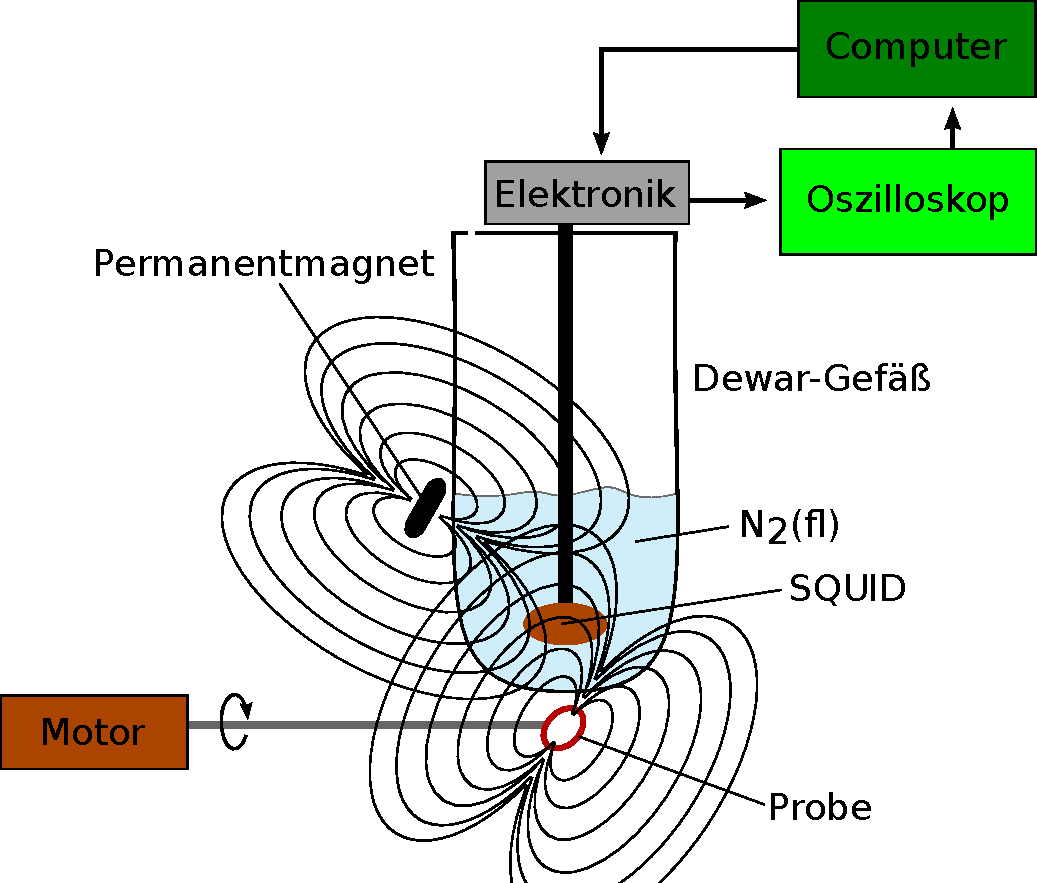
\includegraphics[width=0.95\textwidth]{../img/aufbau.pdf}
  \caption{Aufbau zur Bestimmung des Mitführungskoeffizinenten von Quarz mit einem Ringlaser.}
  \label{img:aufbau}
\end{center}
\end{figure}
\autoref{img:aufbau} zeigt den Aufbau des Ringlasers,
mit dem die Messungen durchgeführt werden.
Um eine Helium-Neon-Röhre,
die von einem statischen elektrischen Feld gepumpt wird,
ist mit drei Spiegeln ein Resonator aufgebaut.
Einer der Spiegel ist halbdurchlässig, um den Laserstrahl auszukoppeln.
Ein vierter Spiegel reflektiert den im Uhrzeigersinn umlaufenden Stahl so,
dass er zusammen mit dem anderen auf eine Photodiode fällt.
Der vierte Spiegel und der Halbdurchlässige können in ihrer Position verändert werden.
Im Strahlengang befindet sich außerdem eine einstellbare Blende,
mit welcher der Strahl abgeschwächt werden kann.
Zusätzlich sind im Strahlengang zwei Quarzscheiben,
die im Brewsterwinkel vom Laserstrahl getroffen werden.
Eine davon kann mit einem Motor in Rotation versetzt und ihre Drehzahl $\omega$ gemessen werden.
Der Laserstrahl trifft im Abstand $x_0$ von der vertikalen Achse der Scheibe auf.
Die zweite, ruhende Scheibe ist dazu da,
den abgelenkten Strahl wieder zurück in den ursprünglichen Strahlverlauf zu brechen.\\
Das Signal der Photodiode wird auf einem Oszilloskop angezeigt und kann
vom Computer ausgelesen werden. \\[\baselineskip]
Technische Daten des Versuchaufbaus:
\begin{itemize}
  \item optische Länge des Resonators: $L = 214.9$\,cm
  \item Wellenlänge des He-Ne-Laser in Luft: $\lambda = 632.8$\,nm
  \item Brechungsindex von Quarzglas: $n = 1.457$
  \item Dicke der Quarzscheibe: $d = 1.27$\,cm
\end{itemize}
\section{Experimental Procedure}
Chronologische Dokumentation des Ablaufes und der Messdaten.
\section{Messergebnisse und Auswertung}

\subsection{Energieeichung des MCAs}
\begin{figure}[H]
\begin{center}
  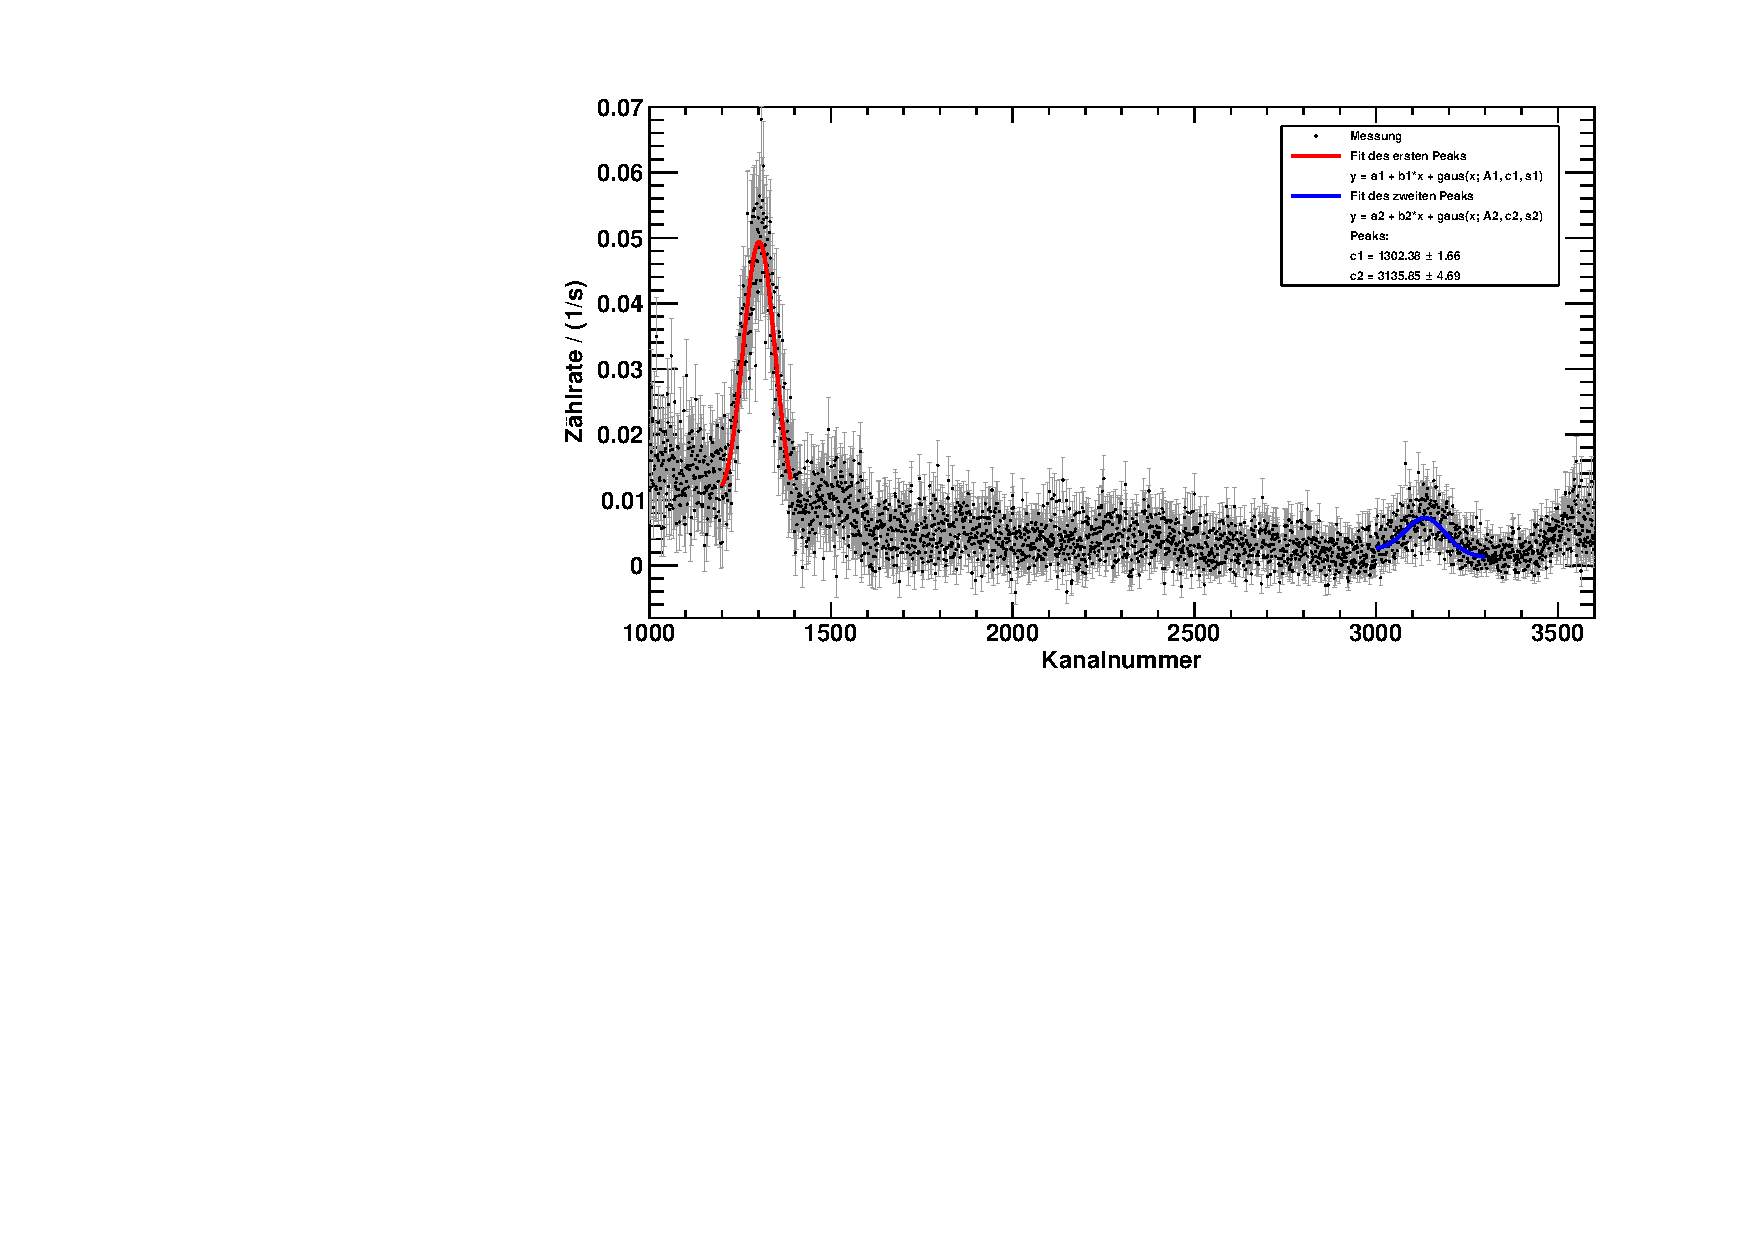
\includegraphics[width=\textwidth]{../img/na_peaks.pdf}
  \caption{\textgamma-Spektrum von \chemel{Na}{22} mit 511\,keV Peak}
  \label{img:na:peak}
\end{center}
\end{figure}

\begin{figure}[H]
\begin{center}
  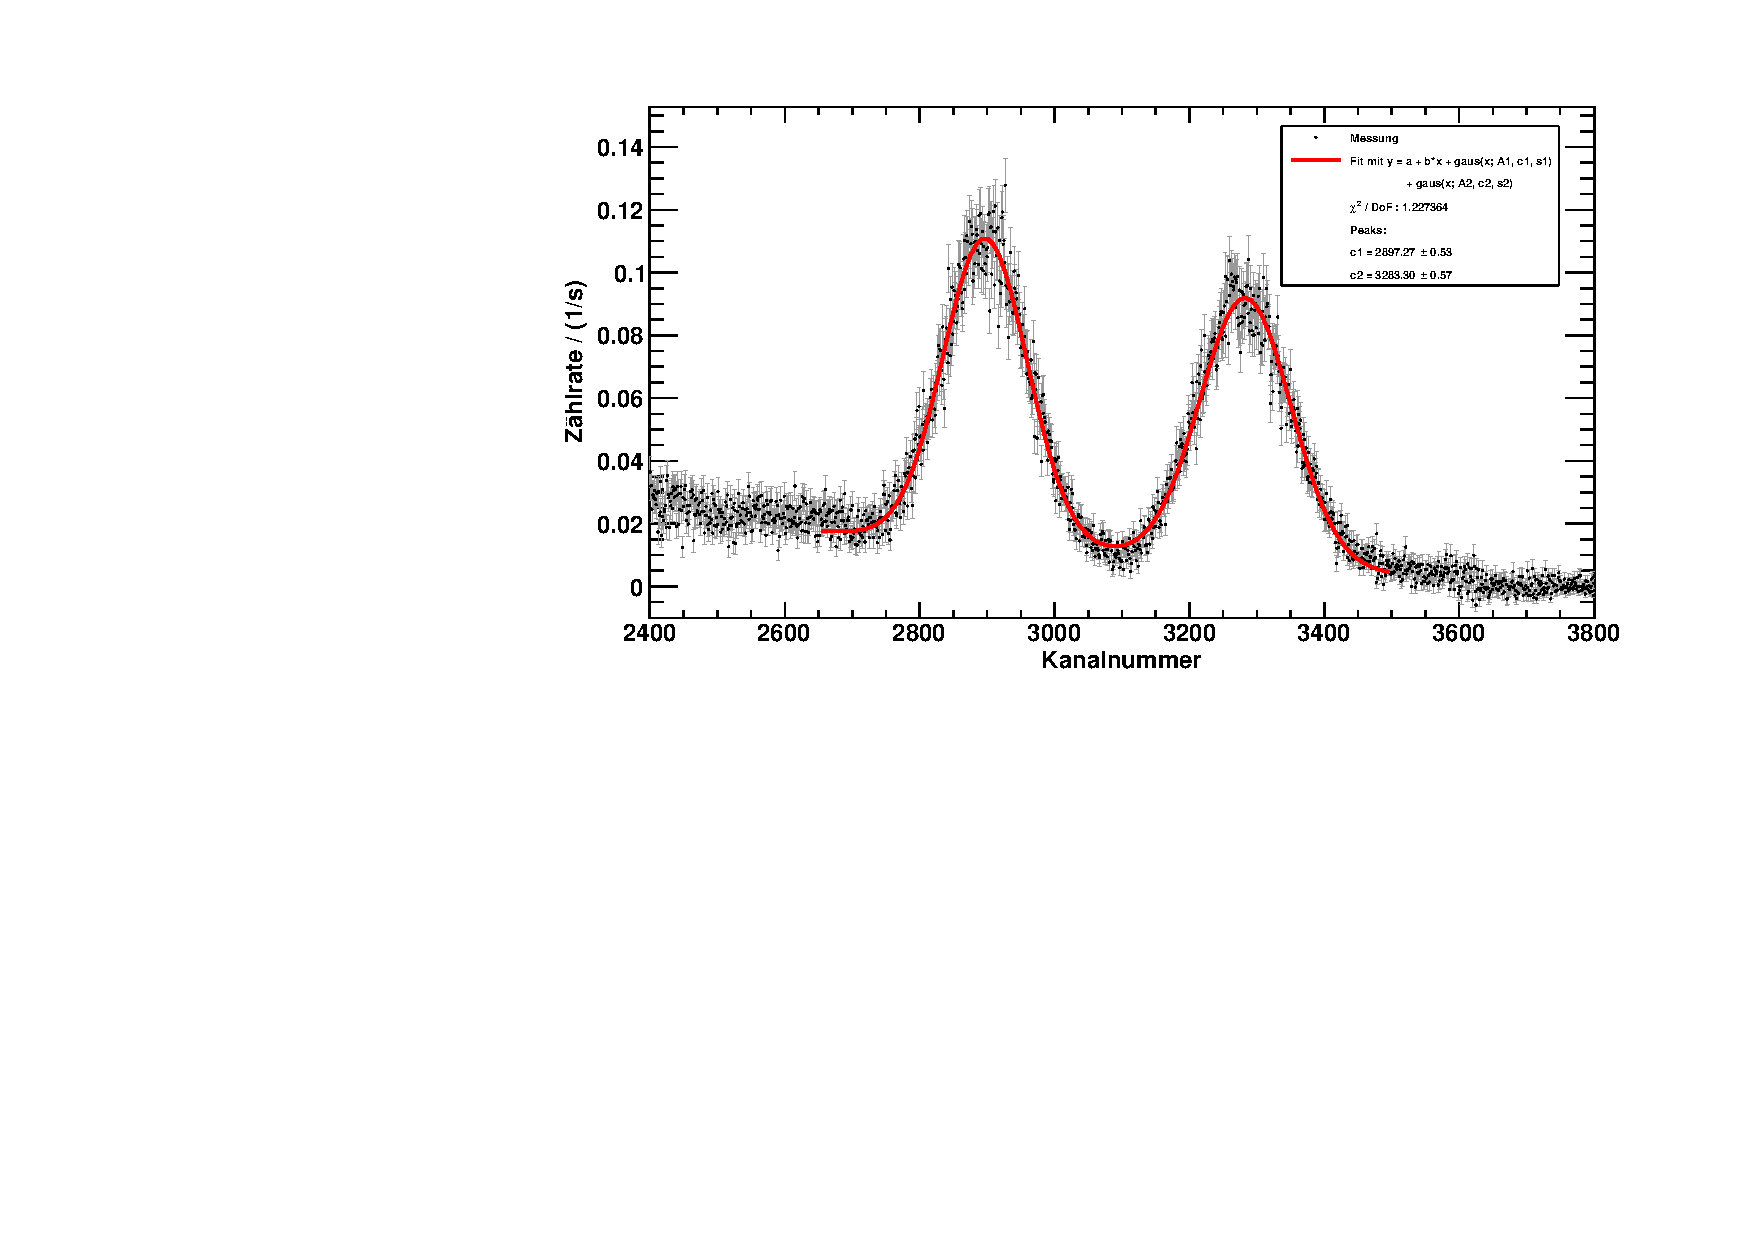
\includegraphics[width=\textwidth]{../img/co_peaks.pdf}
  \caption{\textgamma-Spektrum von \chemel{Co}{60}}
  \label{img:co:peak}
\end{center}
\end{figure}

\begin{figure}[H]
\begin{center}
  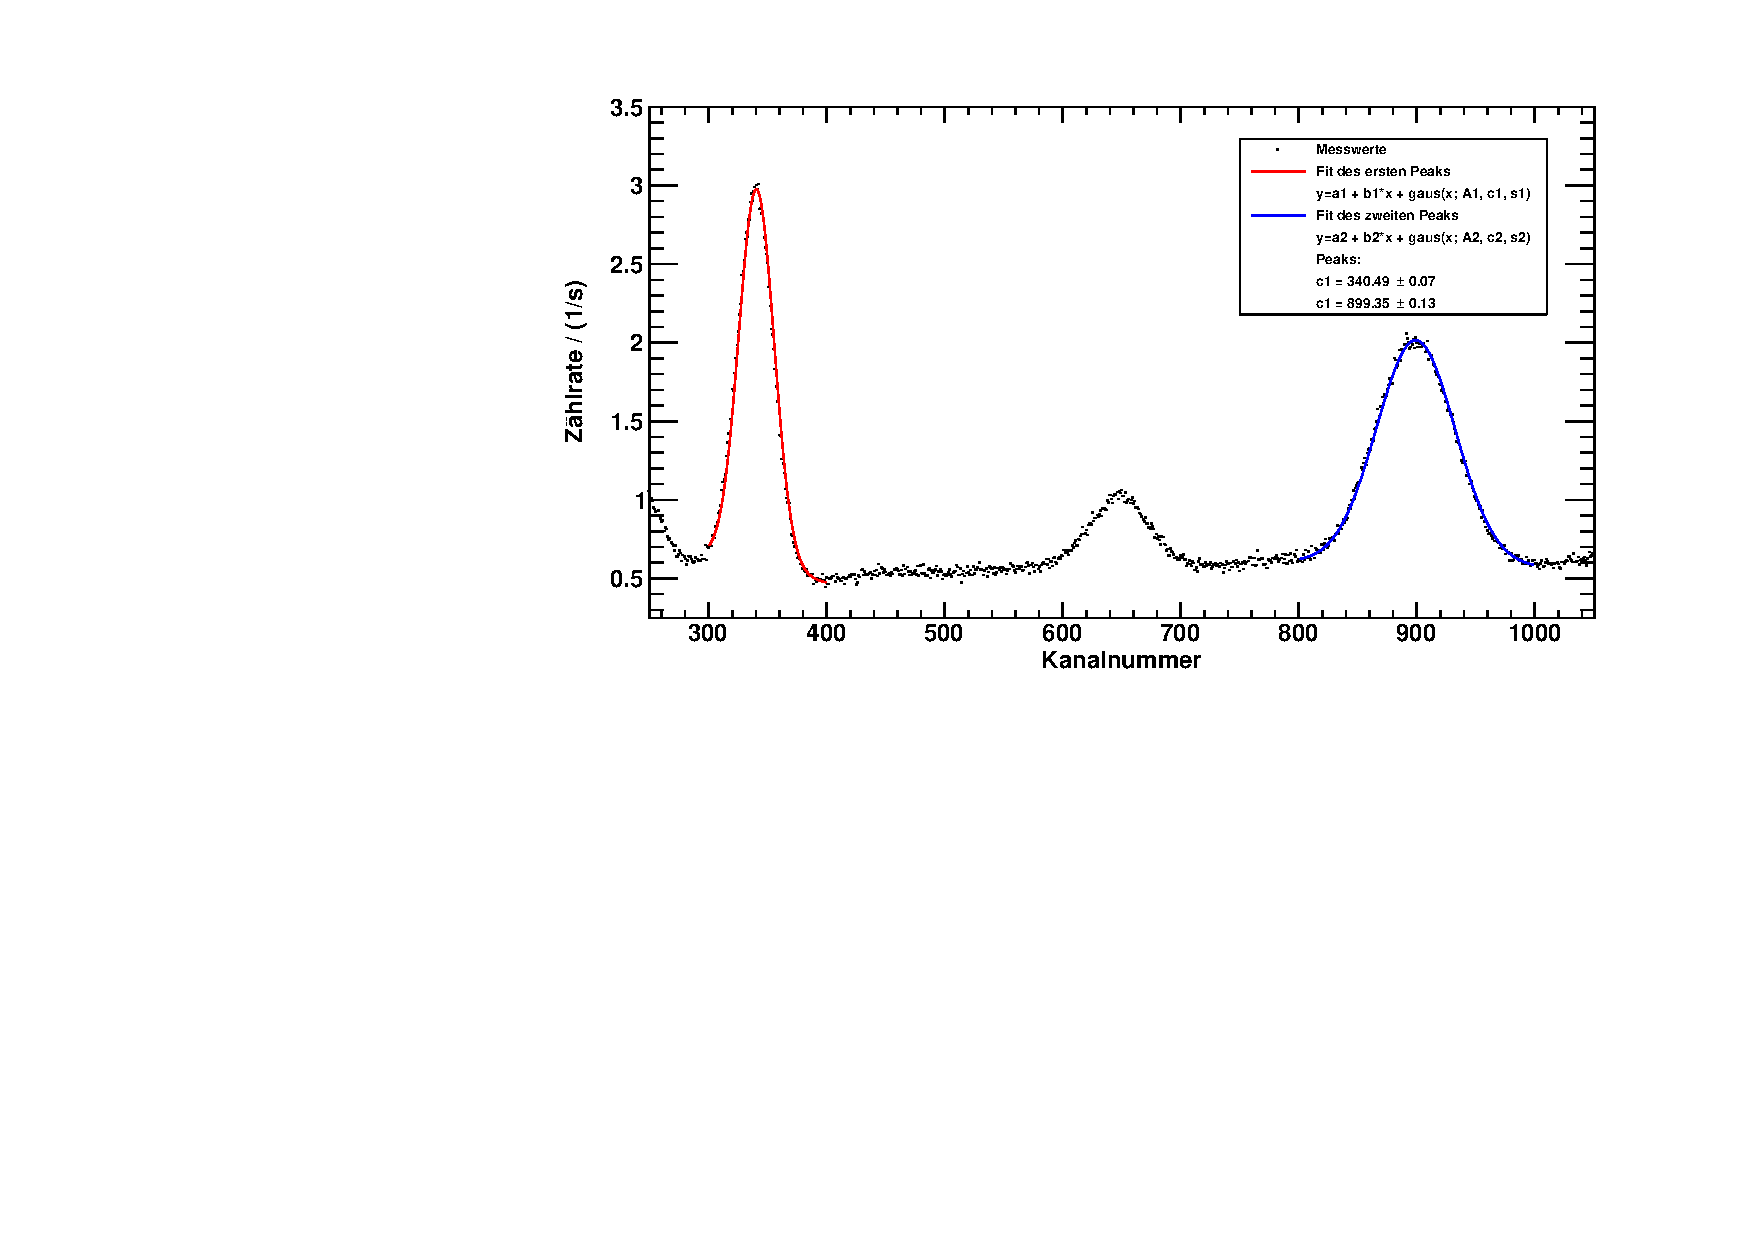
\includegraphics[width=\textwidth]{../img/eu_peaks.pdf}
  \caption{\textgamma-spektrum von \chemel{Eu}{152}}
  \label{img:eu:peak}
\end{center}
\end{figure}

\begin{figure}[H]
\begin{center}
  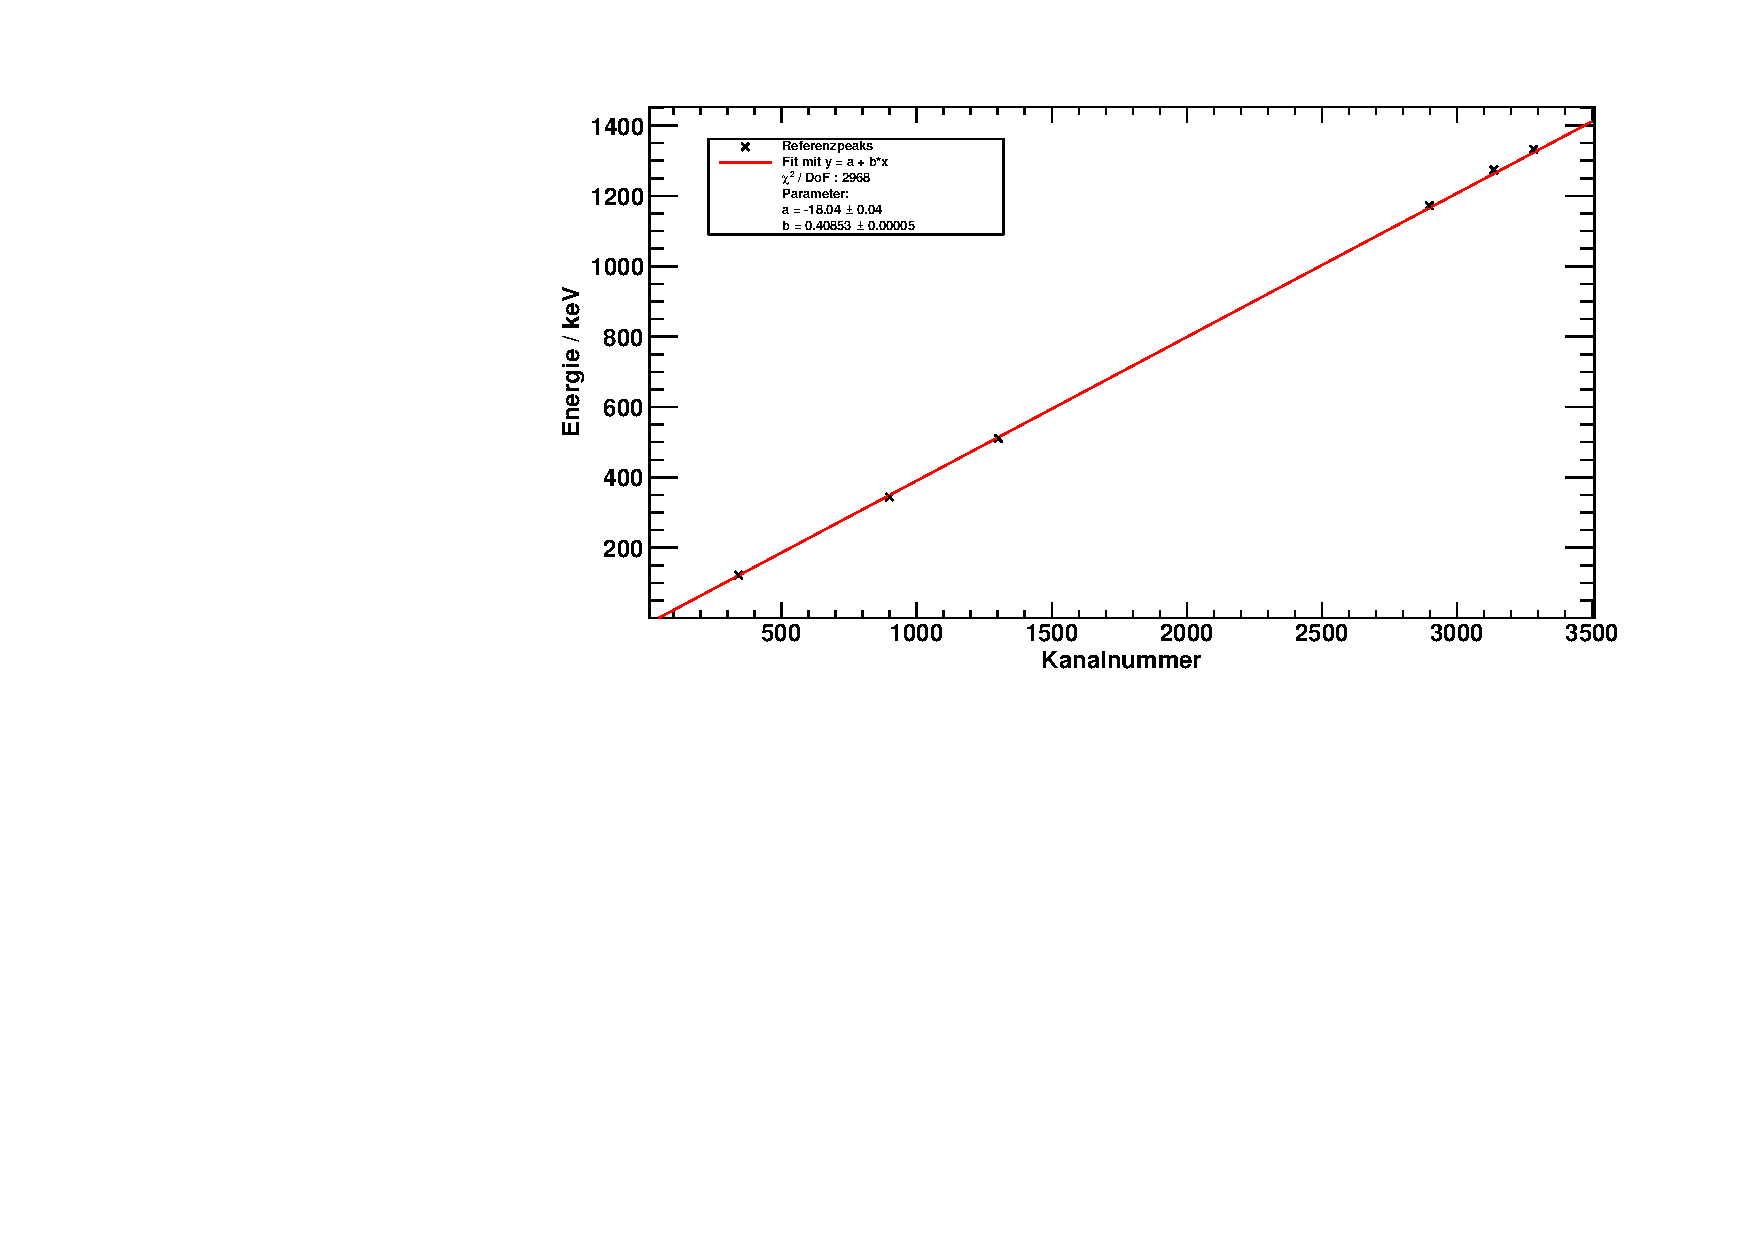
\includegraphics[width=\textwidth]{../img/energy_gauge_lin.pdf}
  \caption{Lineare Energieeichung}
  \label{img:gauge:lin}
\end{center}
\end{figure}

\begin{figure}[H]
\begin{center}
  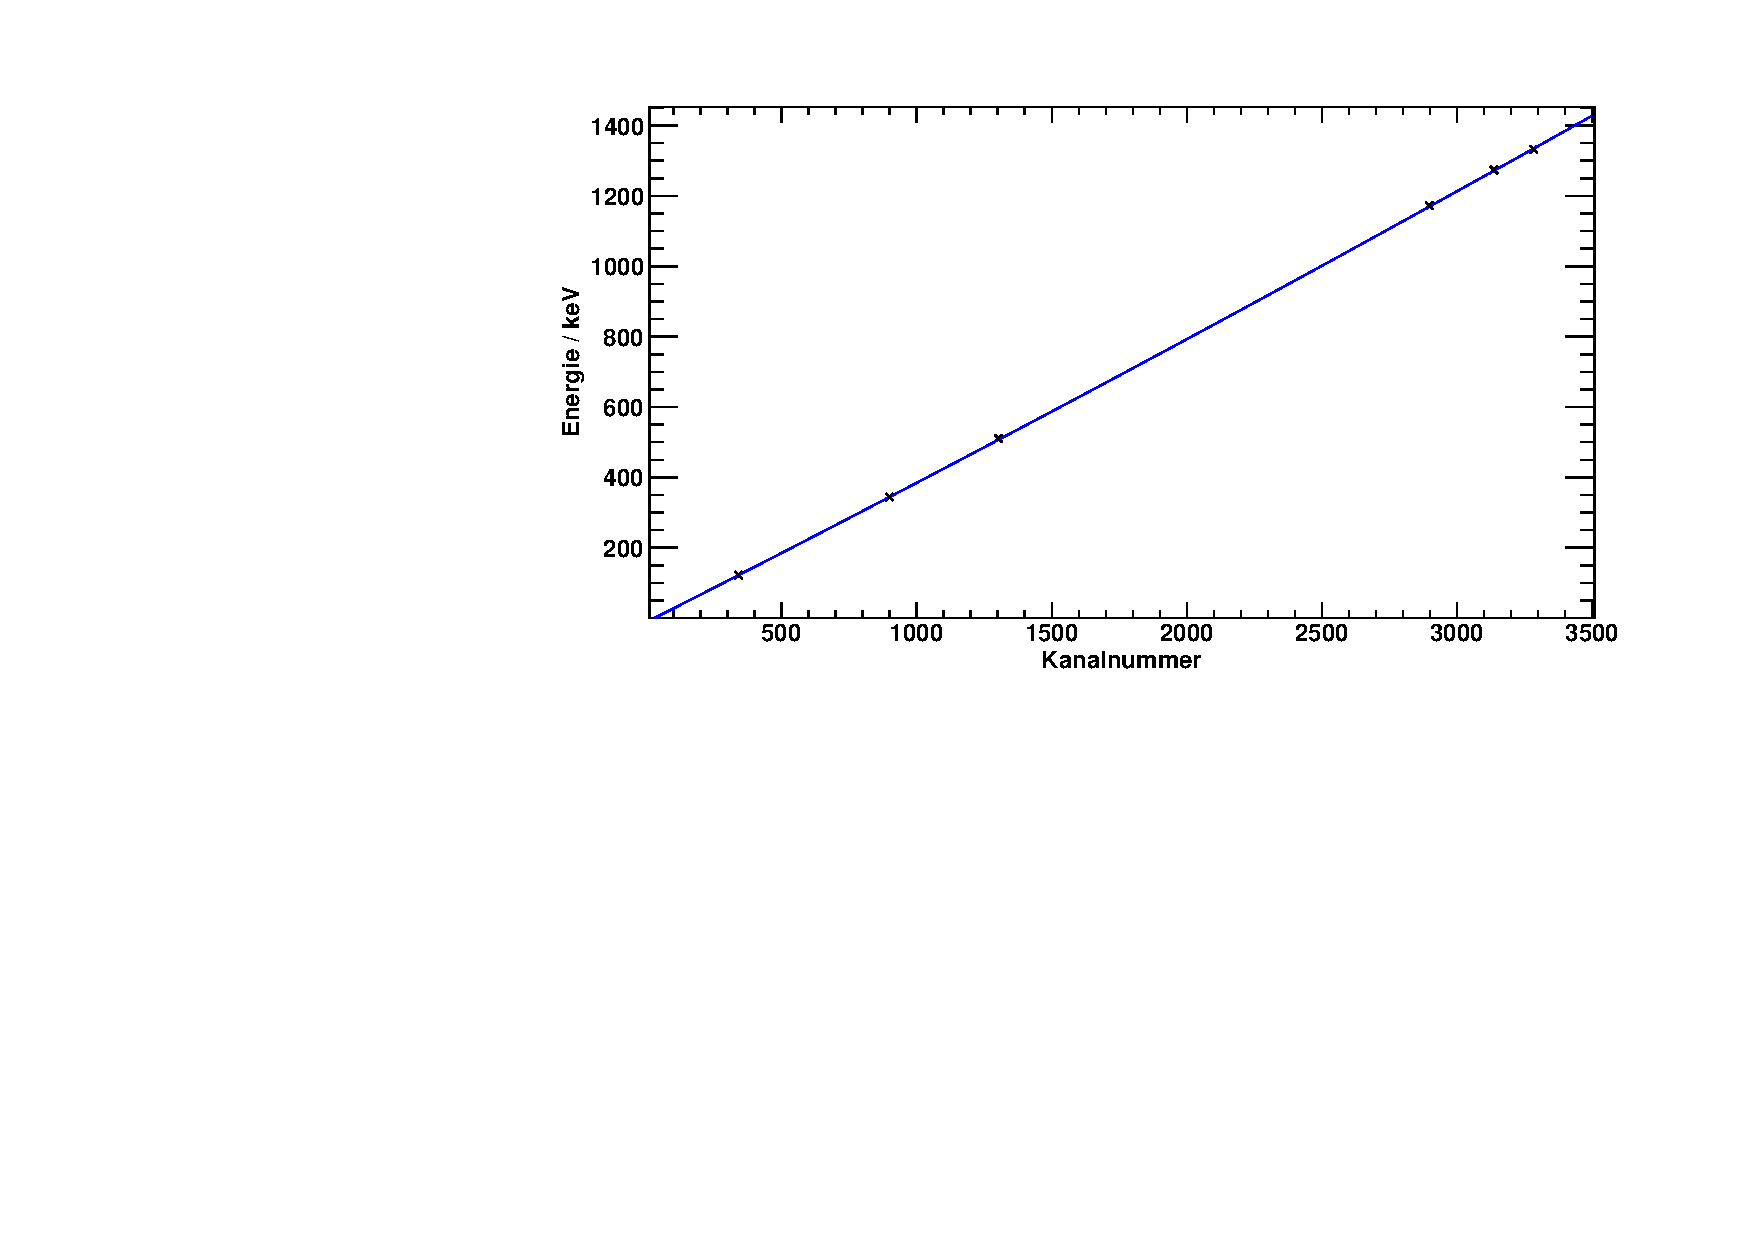
\includegraphics[width=\textwidth]{../img/energy_gauge_quad.pdf}
  \caption{Quadratische Energieeichung}
  \label{img:gauge:lin}
\end{center}
\end{figure}

\subsection{\textgamma-Spektrum von \chemel{Th}{228}}
\begin{figure}[H]
\begin{center}
  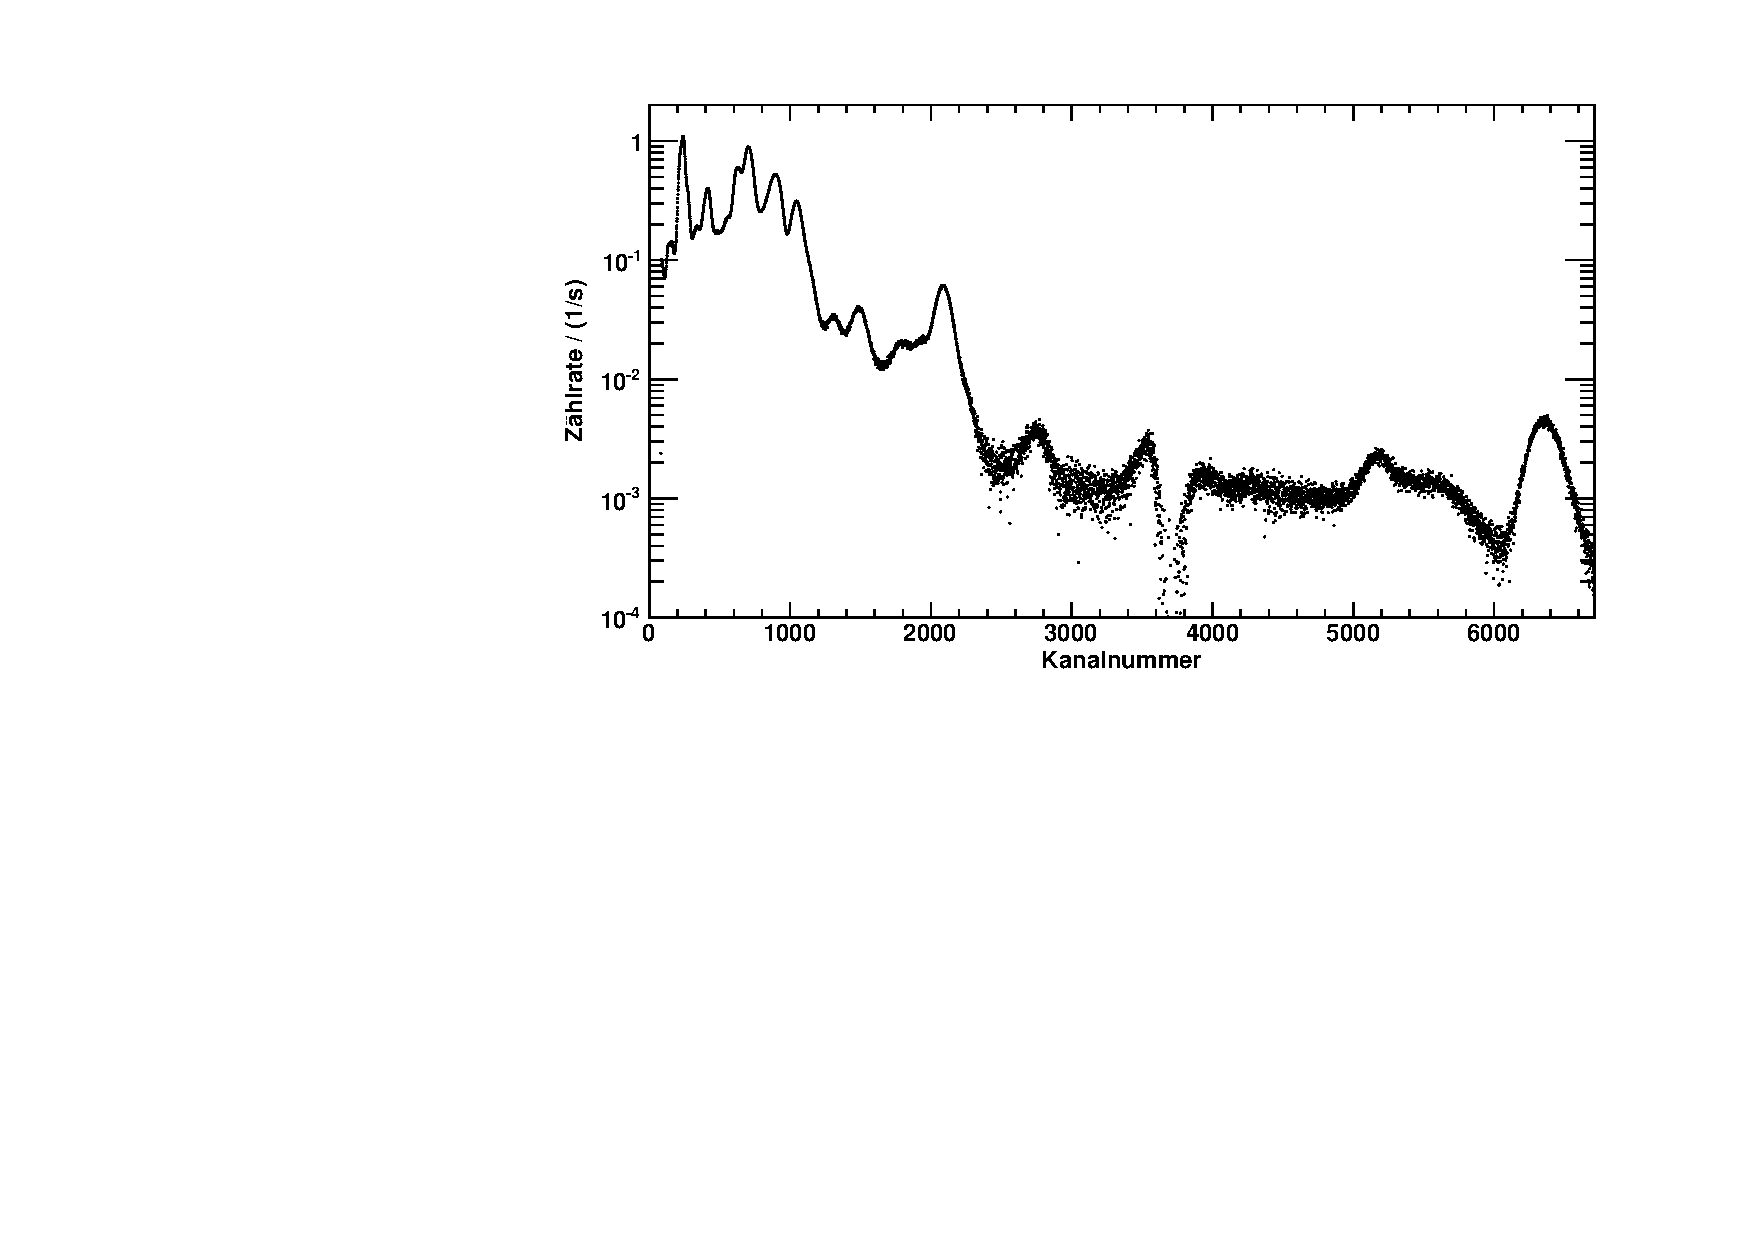
\includegraphics[width=\textwidth]{../img/th_energyspectrum.pdf}
  \caption{\textgamma-Spektrum von \chemel{Th}{228}}
  \label{img:th:spectrum}
\end{center}
\end{figure}

\subsubsection{Single-Peak Fit} % TODO Benennung
\begin{figure}[H]
\begin{center}
  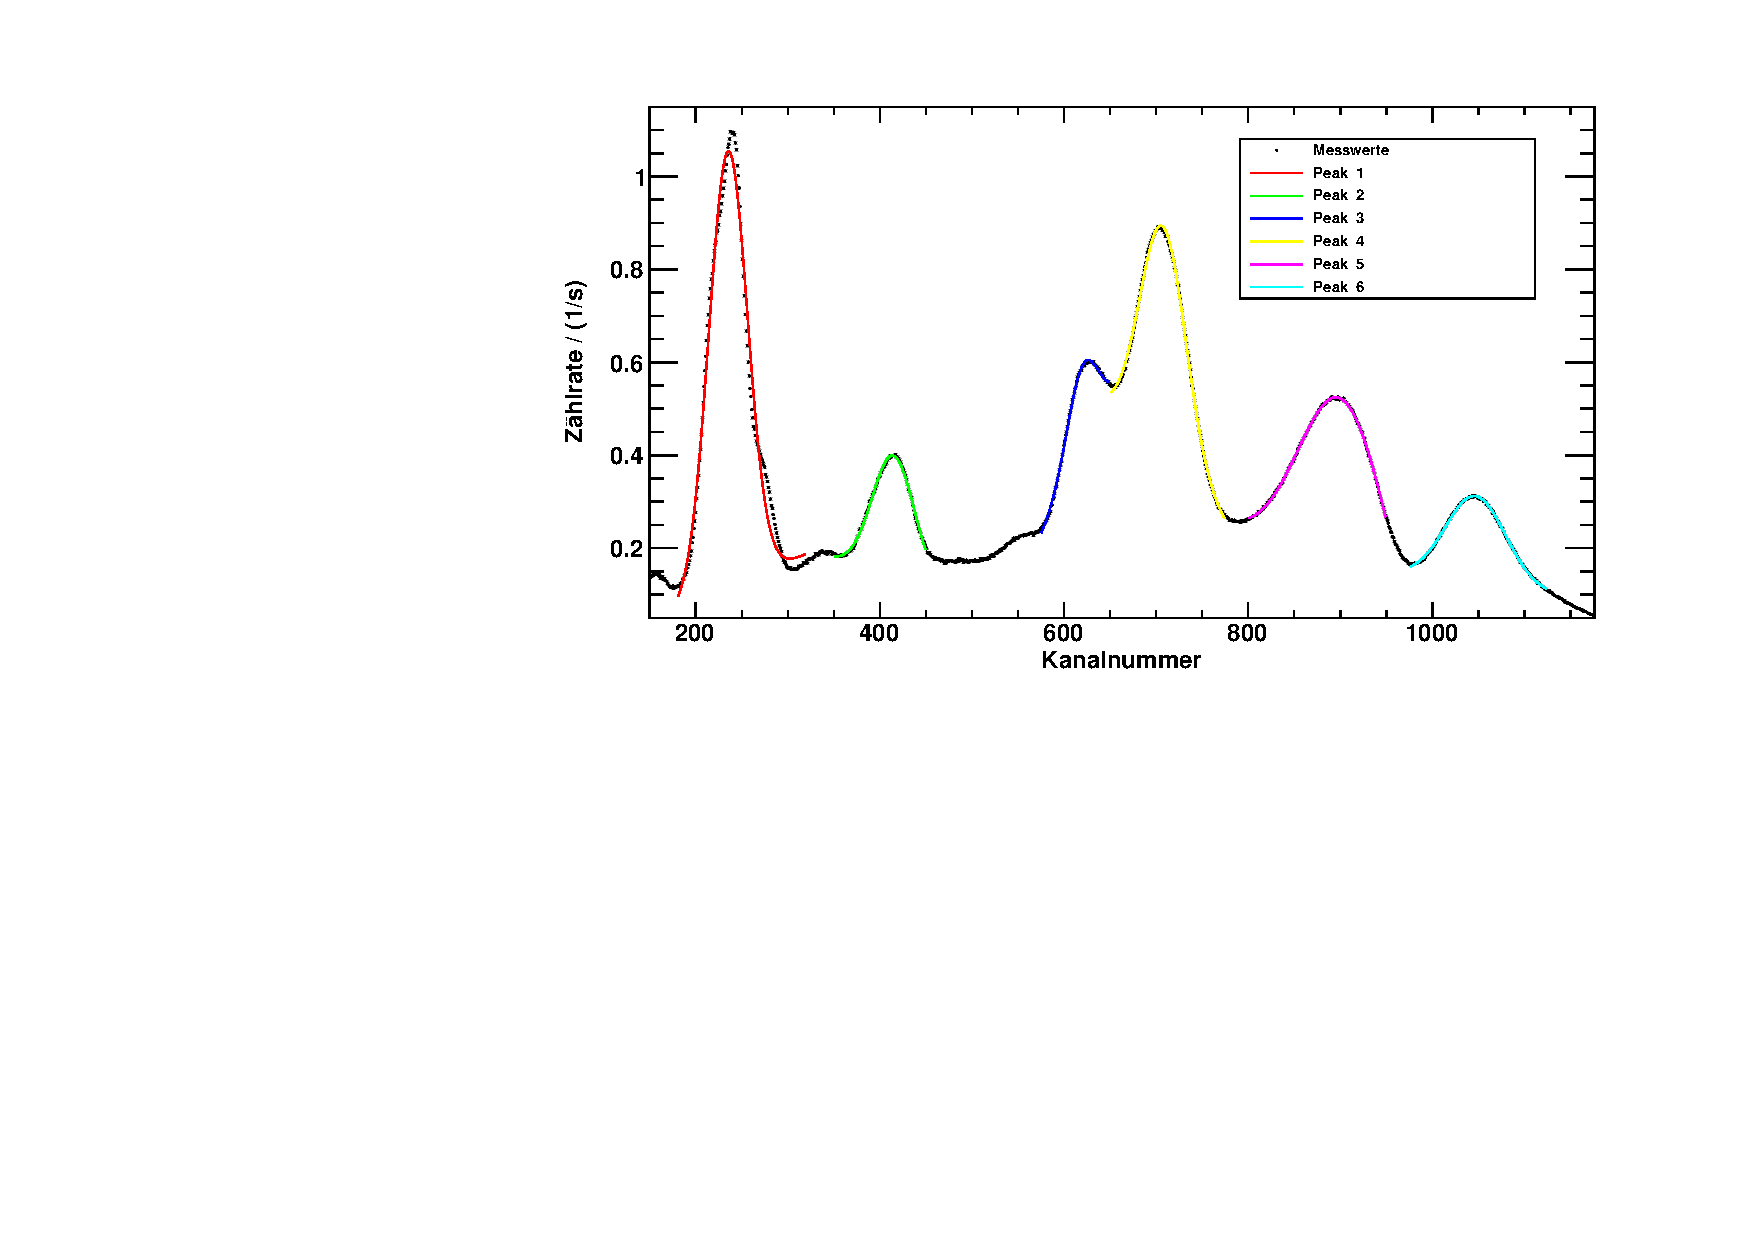
\includegraphics[width=\textwidth]{../img/th_peaks_single_01-06.pdf}
  \caption{Peaks 1 bis 6}
  \label{img:th:peaks:single:0106}
\end{center}
\end{figure}

\begin{figure}[H]
\begin{center}
  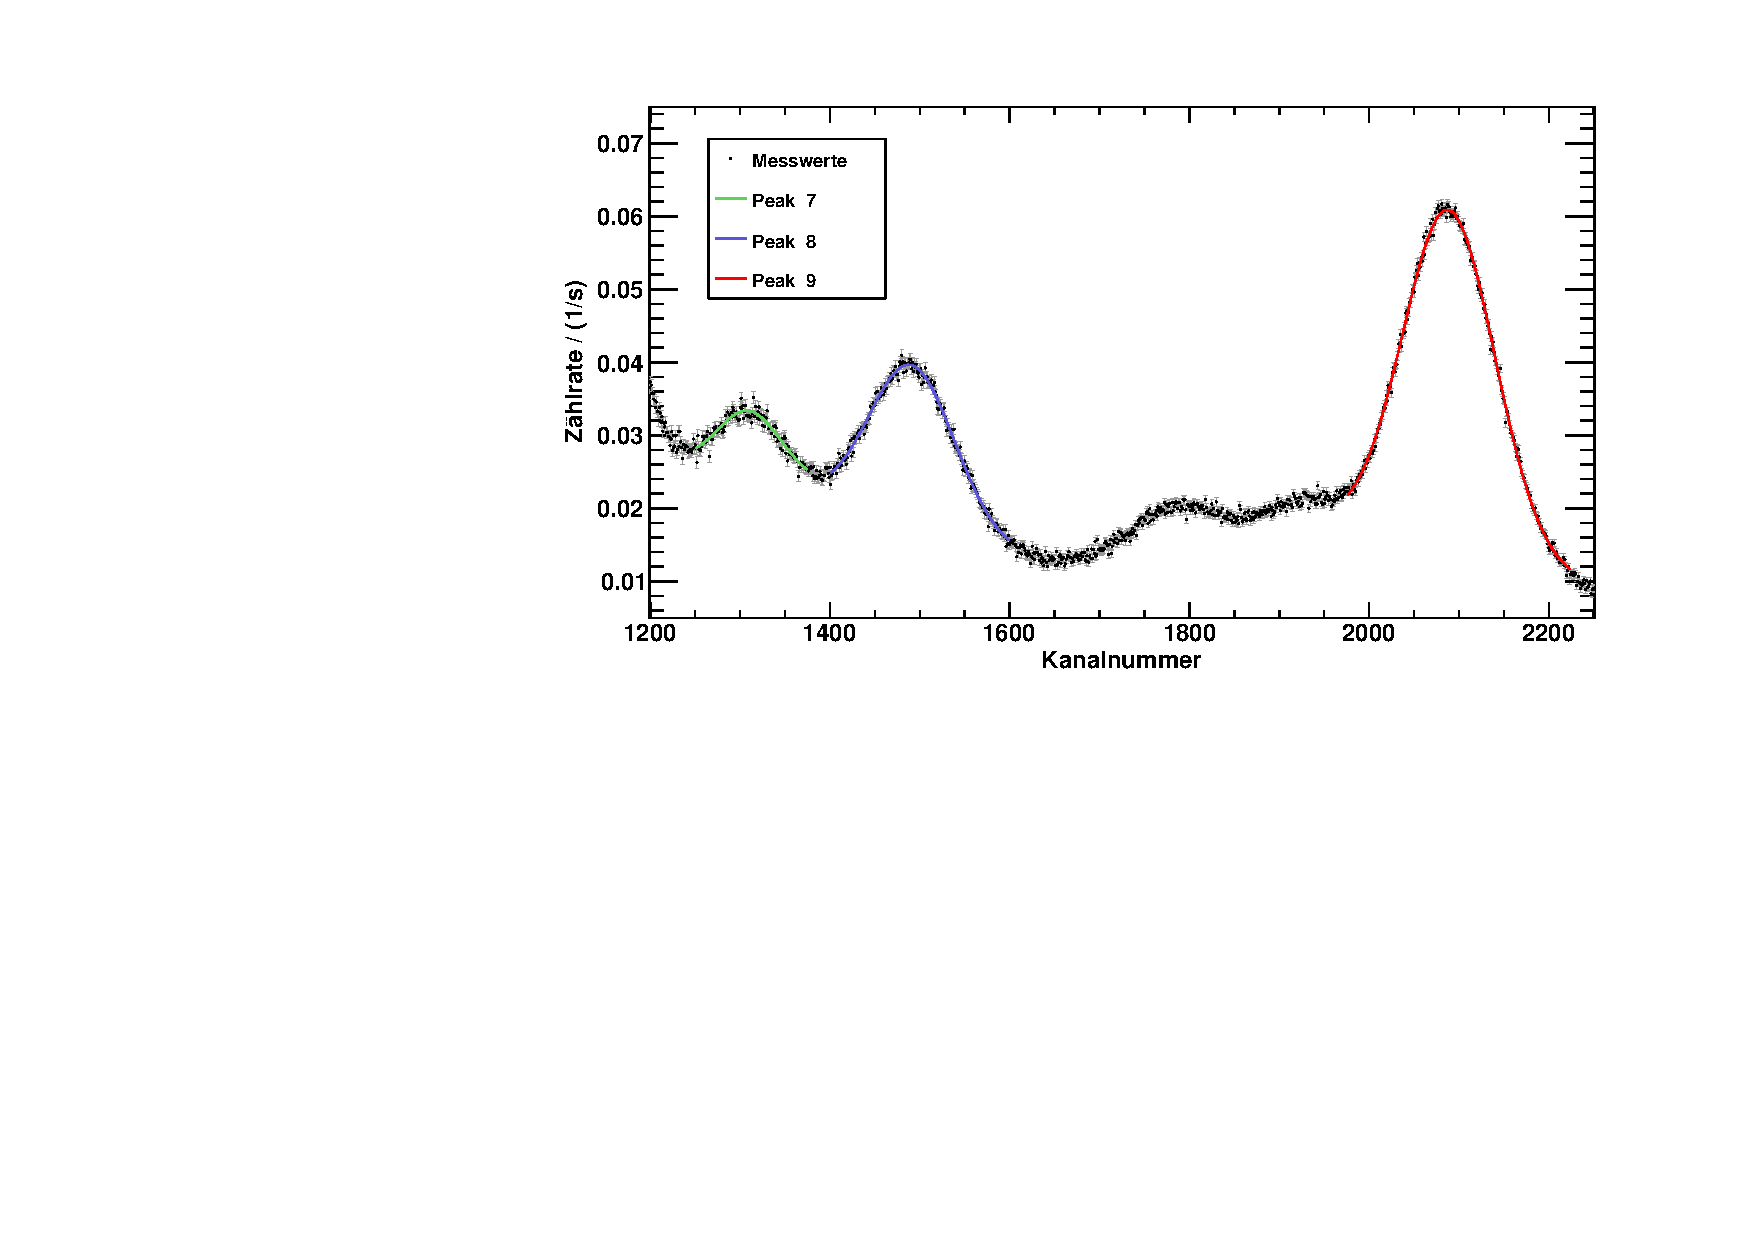
\includegraphics[width=\textwidth]{../img/th_peaks_single_07-09.pdf}
  \caption{Peaks 7 bis 9}
  \label{img:th:peaks:single:0709}
\end{center}
\end{figure}

\begin{figure}[H]
\begin{center}
  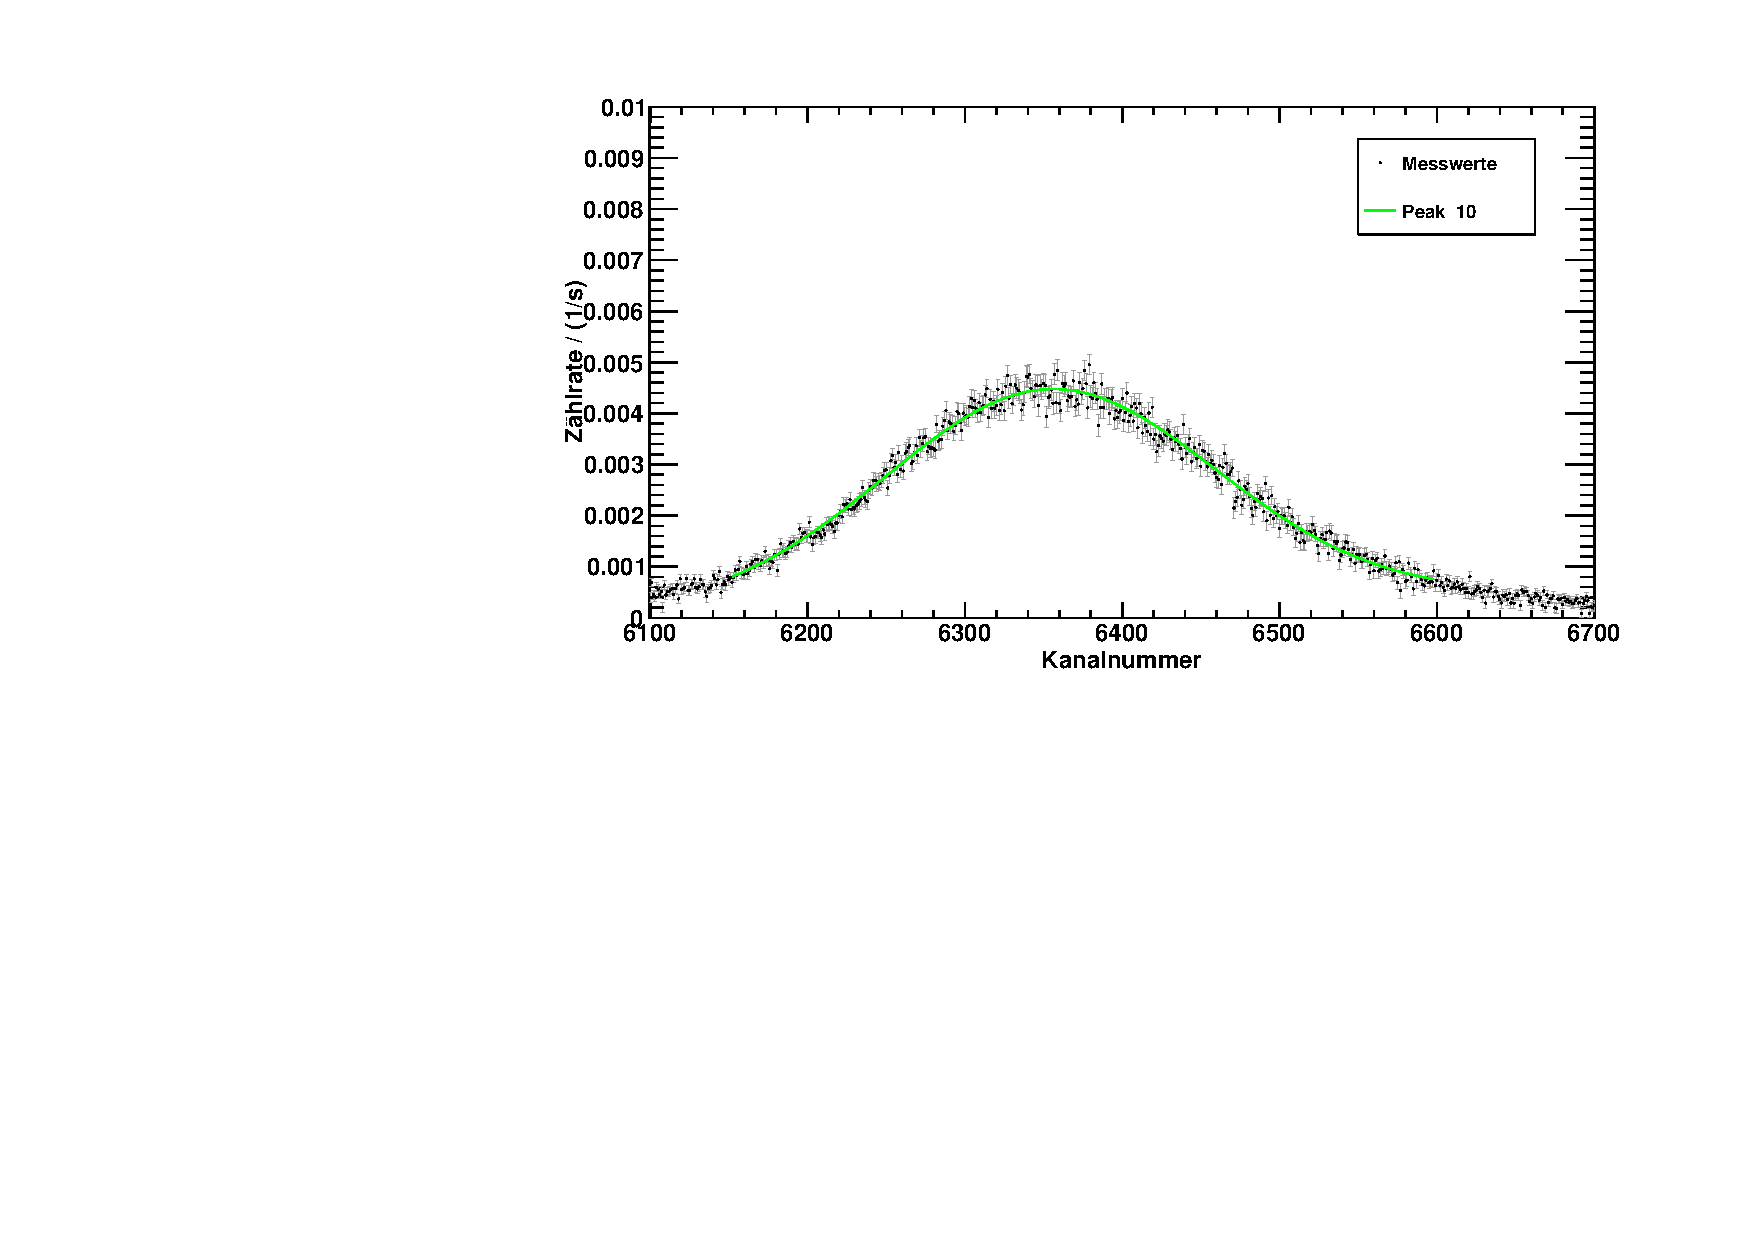
\includegraphics[width=\textwidth]{../img/th_peaks_single_10.pdf}
  \caption{Peak 10}
  \label{img:th:peaks:single:10}
\end{center}
\end{figure}

\subsubsection{Multi-Peak Fit} % TODO Benennung
\begin{figure}[H]
\begin{center}
  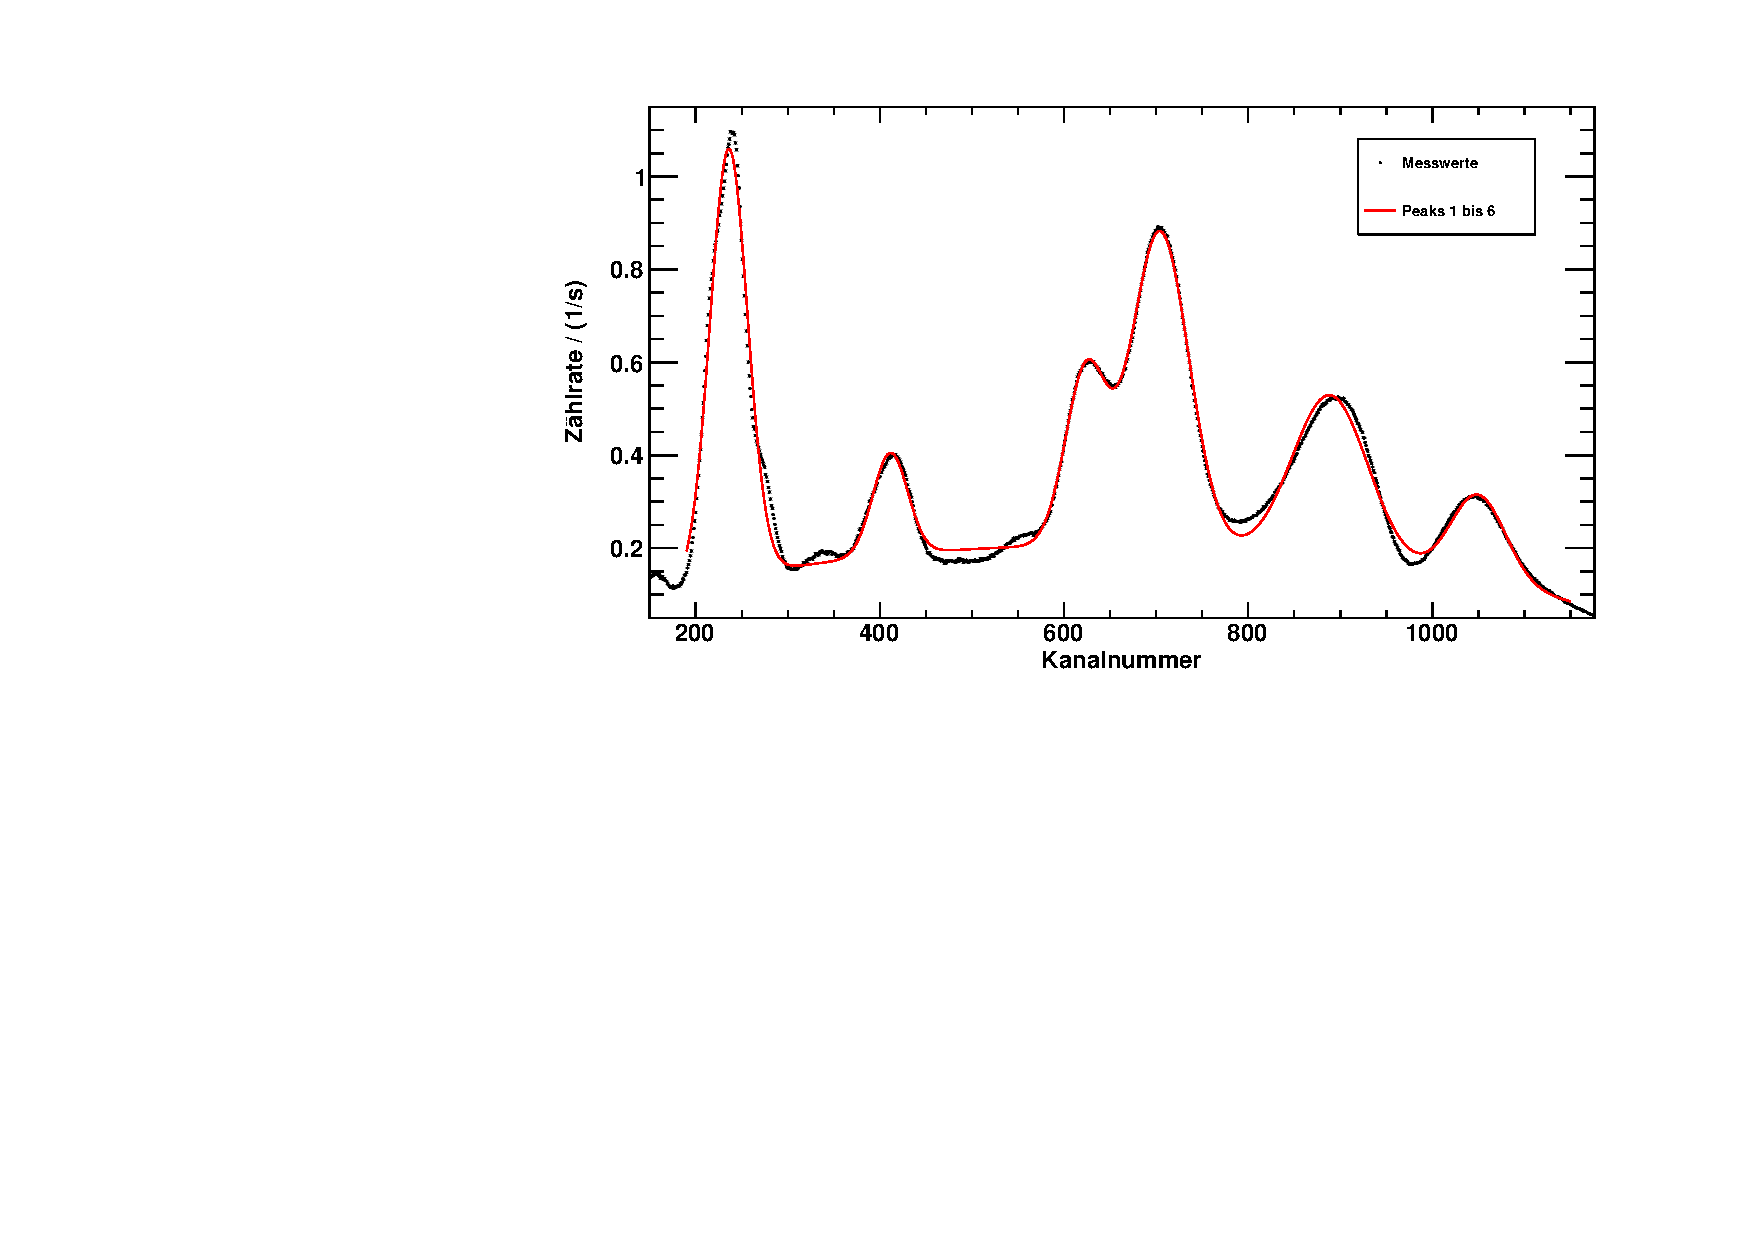
\includegraphics[width=\textwidth]{../img/th_peaks_multi_01-06.pdf}
  \caption{Peaks 1 bis 6}
  \label{img:th:peaks:multi:0106}
\end{center}
\end{figure}

\begin{figure}[H]
\begin{center}
  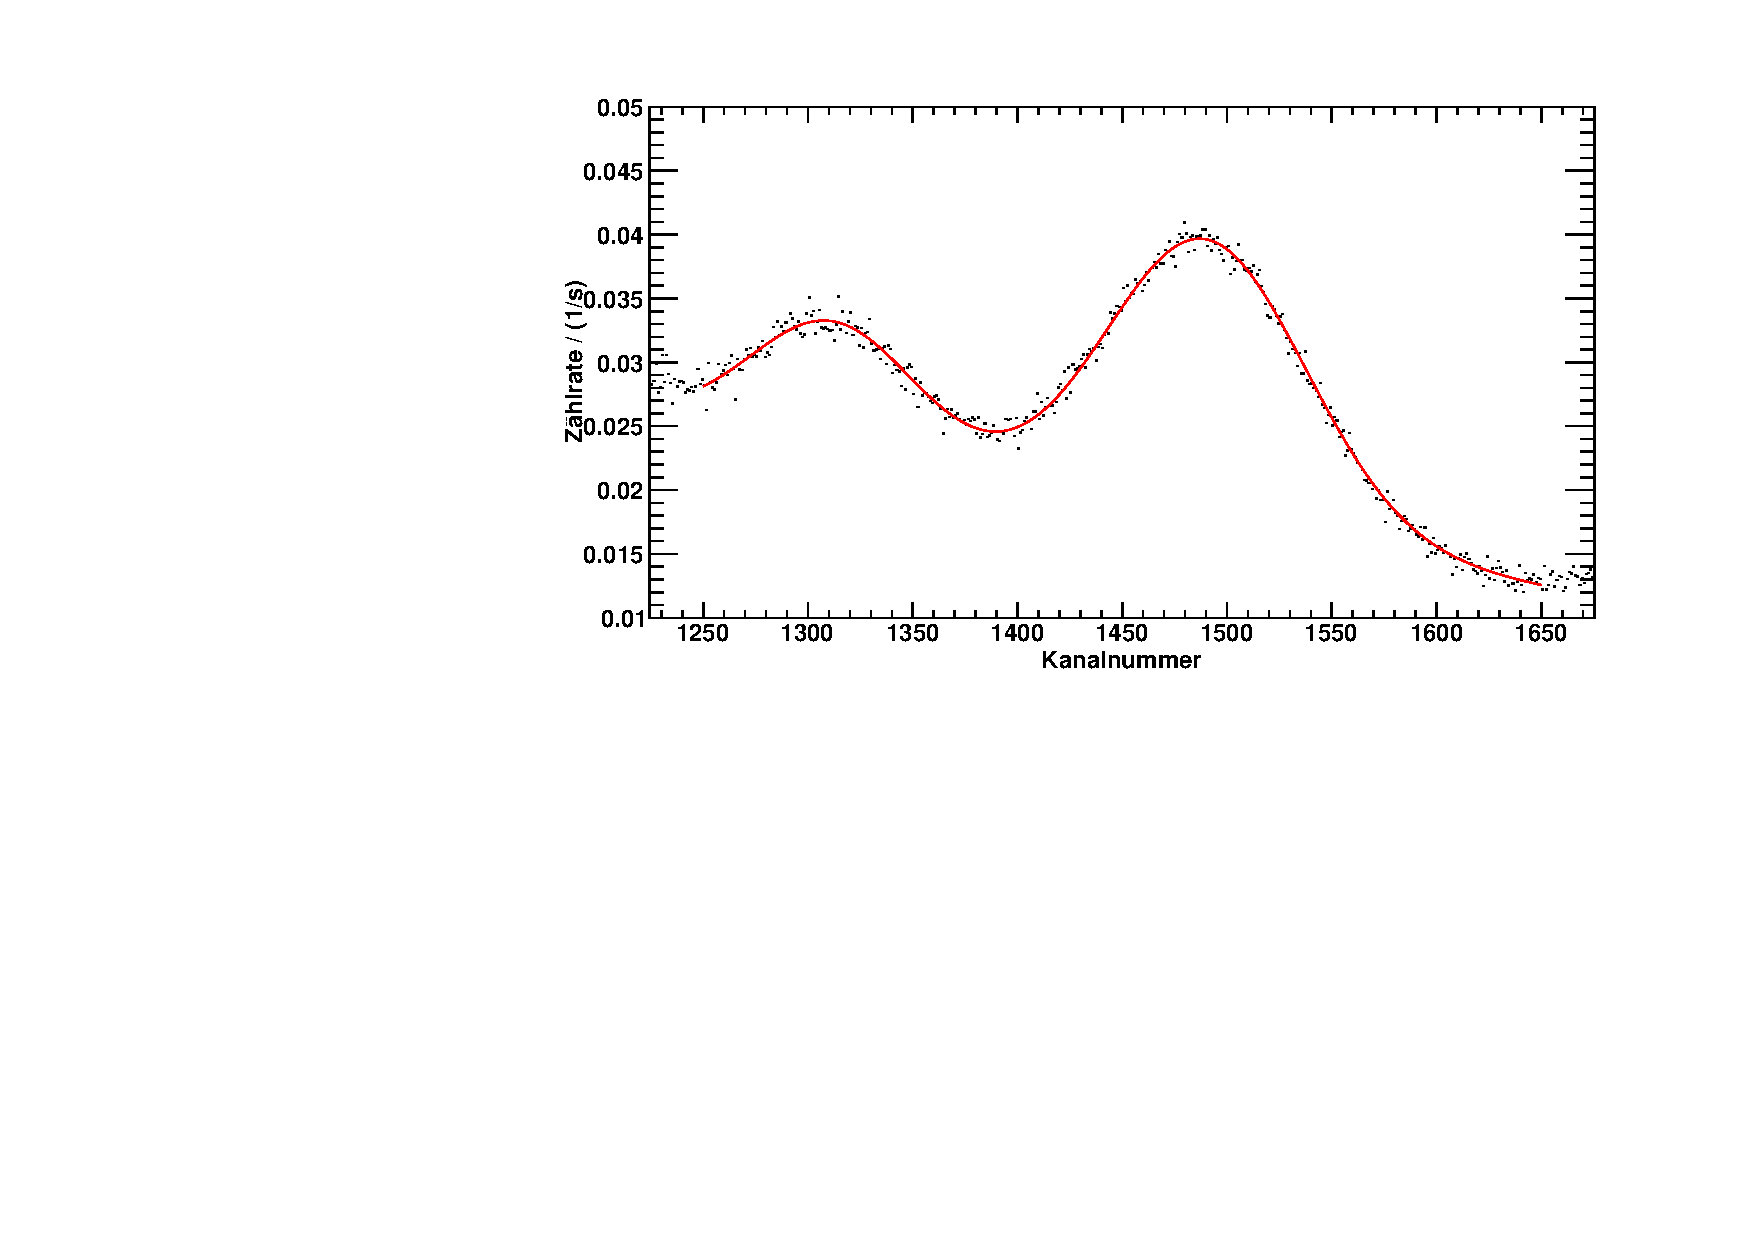
\includegraphics[width=\textwidth]{../img/th_peaks_multi_07-08.pdf}
  \caption{Peaks 7 und 8}
  \label{img:th:peaks:multi:0708}
\end{center}
\end{figure}

\subsection{Untergrund}
\begin{figure}[H]
\begin{center}
  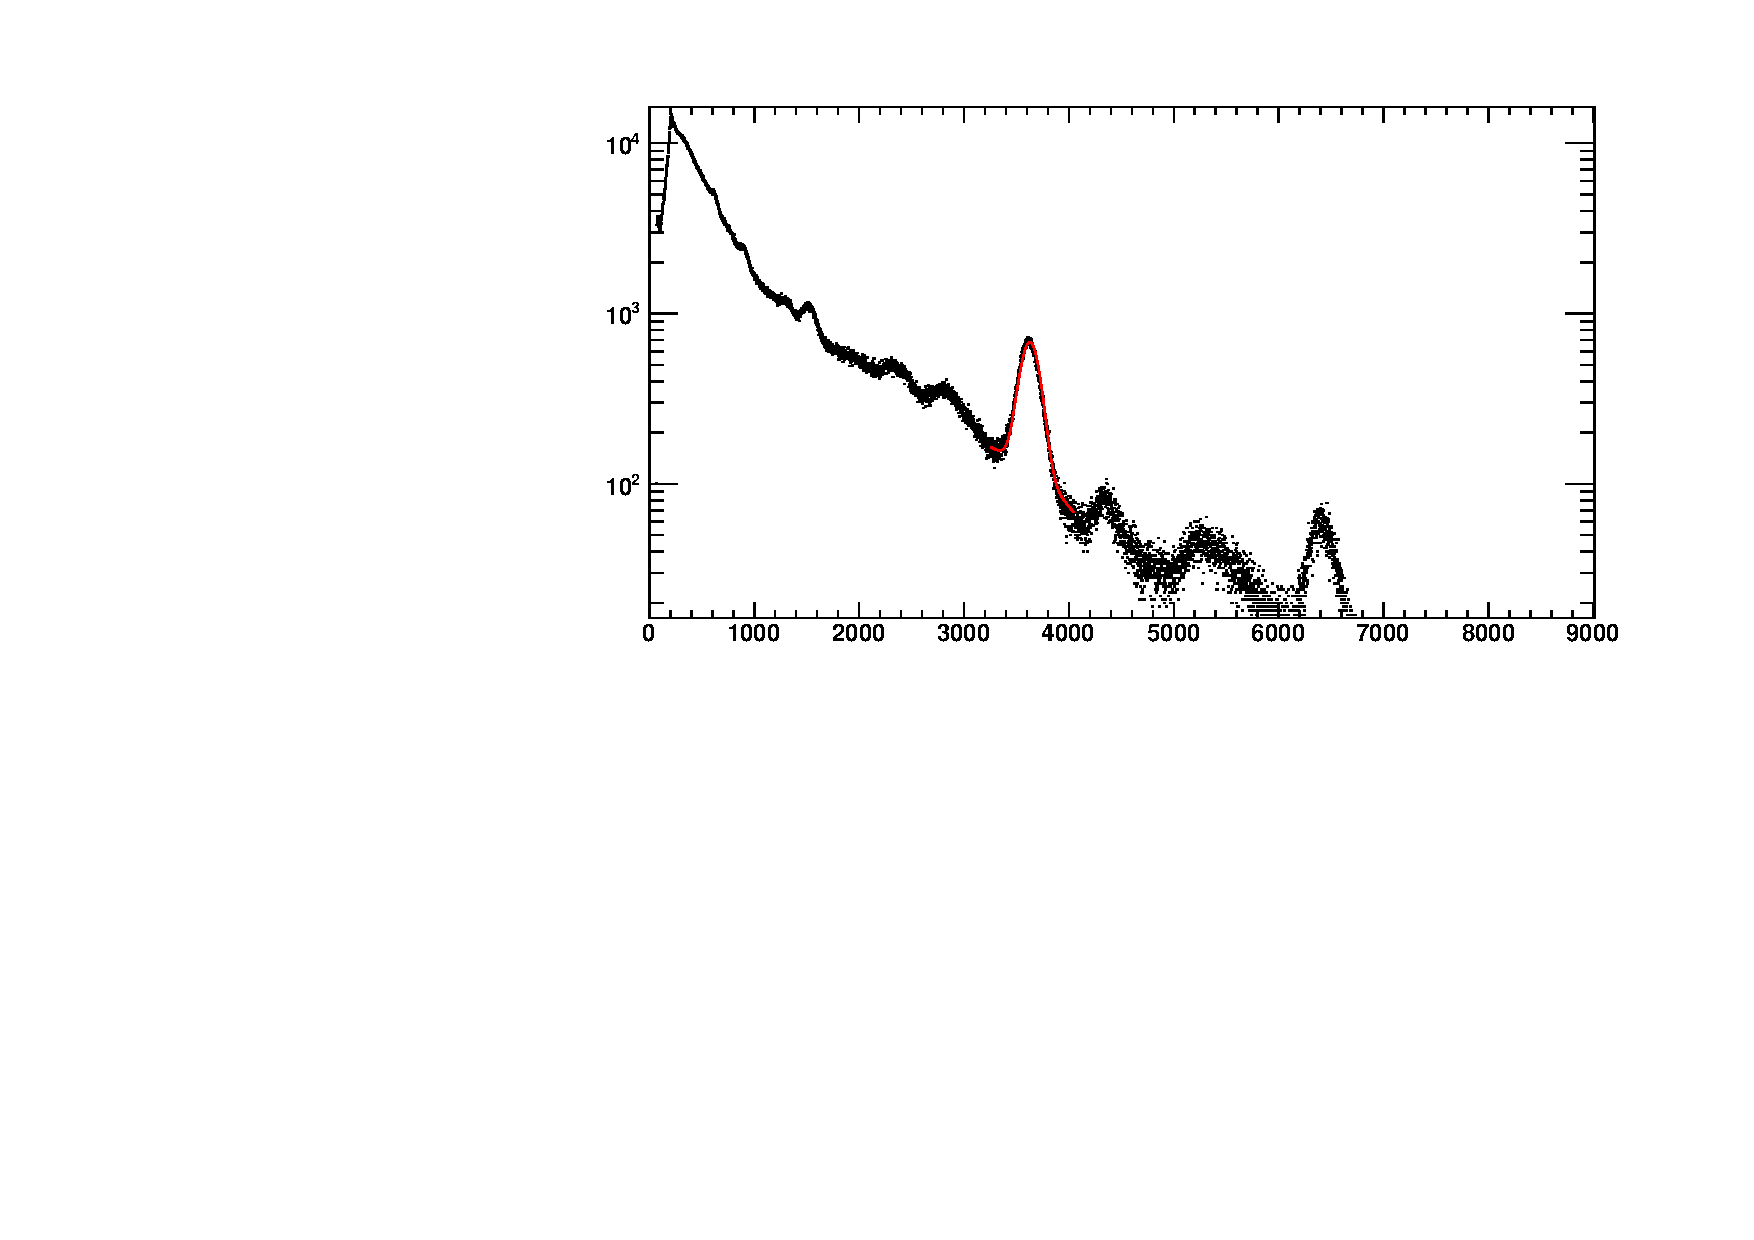
\includegraphics[width=\textwidth]{../img/underground.pdf}
  \caption{Untergrund}
  \label{img:underground}
\end{center}
\end{figure}


\subsection{Winkelkorrelation der \chemel{Na}{22} Vernichtungsphotonen}
\begin{figure}[H]
\begin{center}
  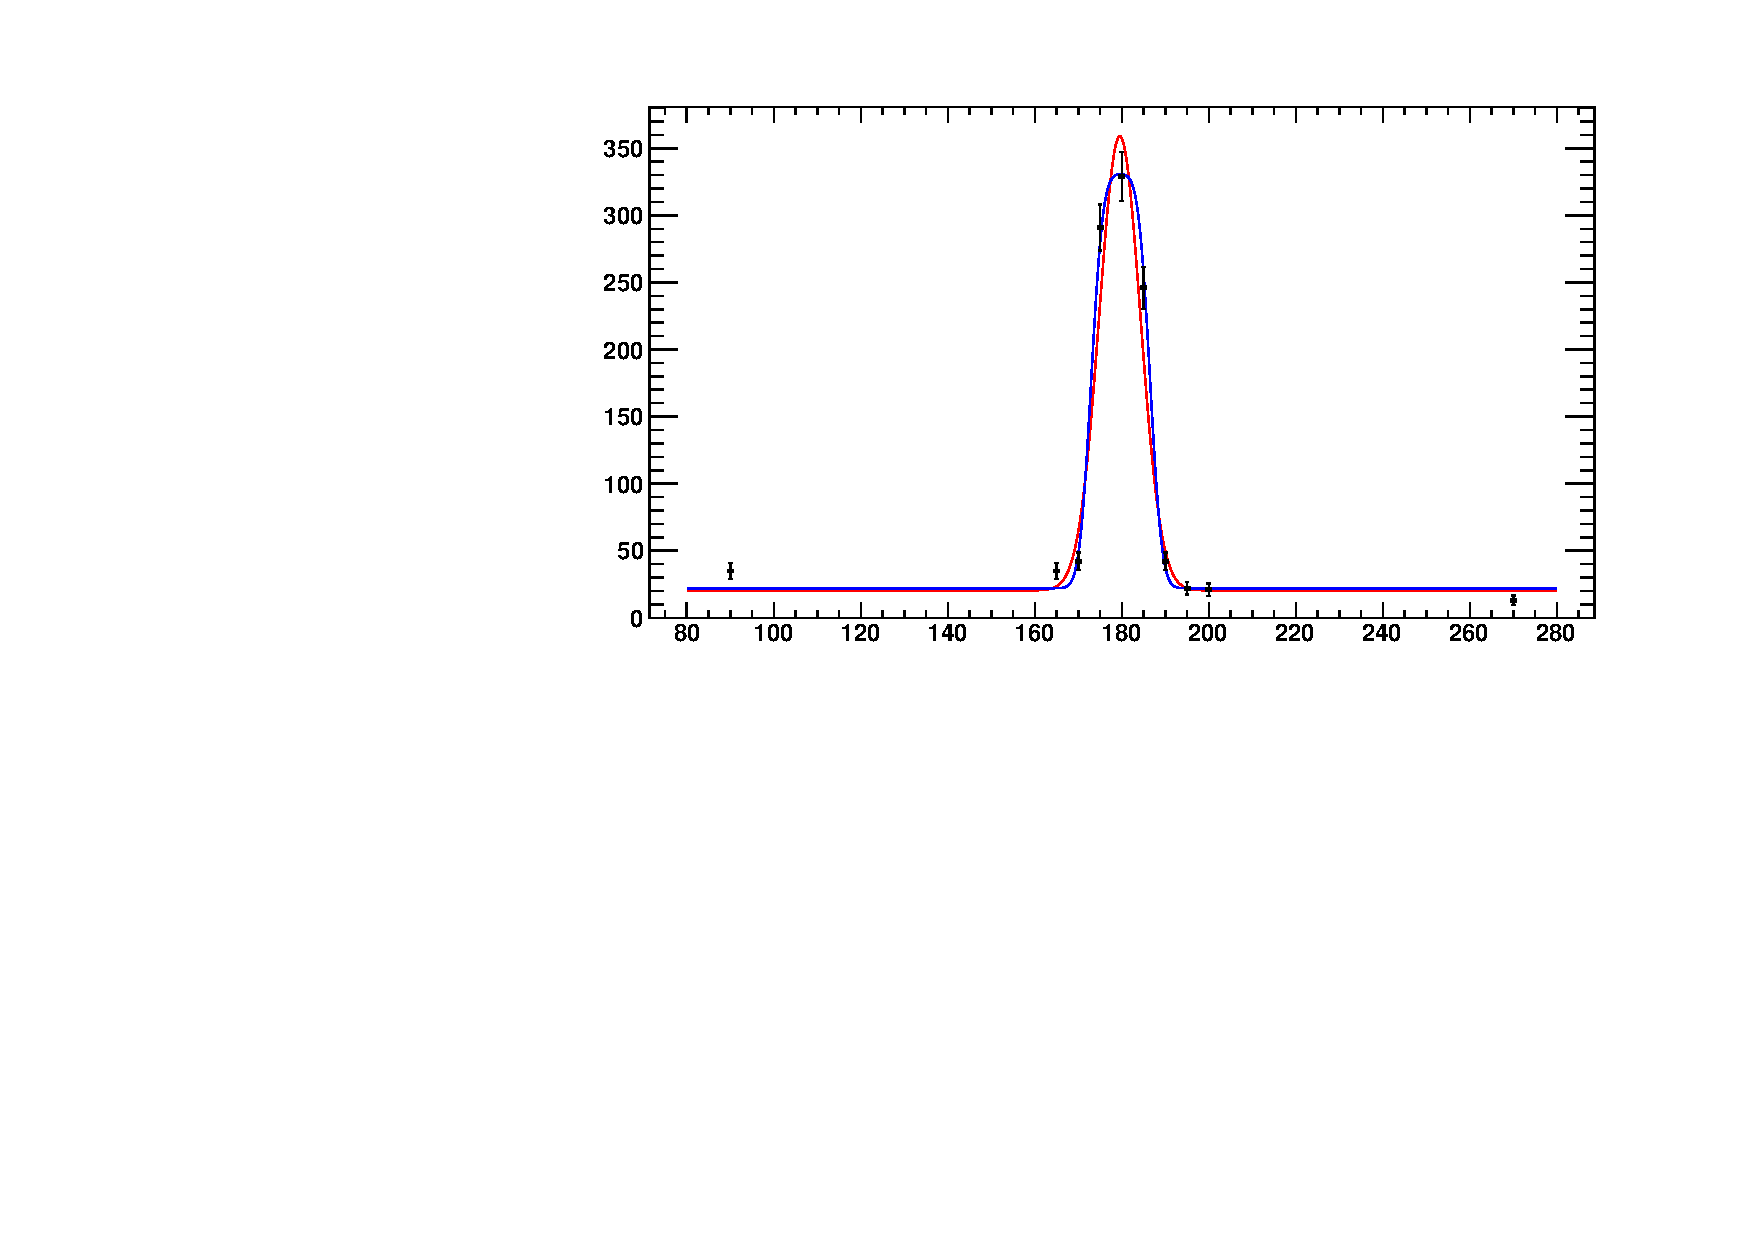
\includegraphics[width=\textwidth]{../img/angles.pdf}
  \caption{Winkelkorrelation der \chemel{Na}{22} Vernichtungsphotonen}
  \label{img:angles}
\end{center}
\end{figure}


%TODO add when finished
%\appendix
%\section{Anhang}
%\subsection{Messprotokoll}
%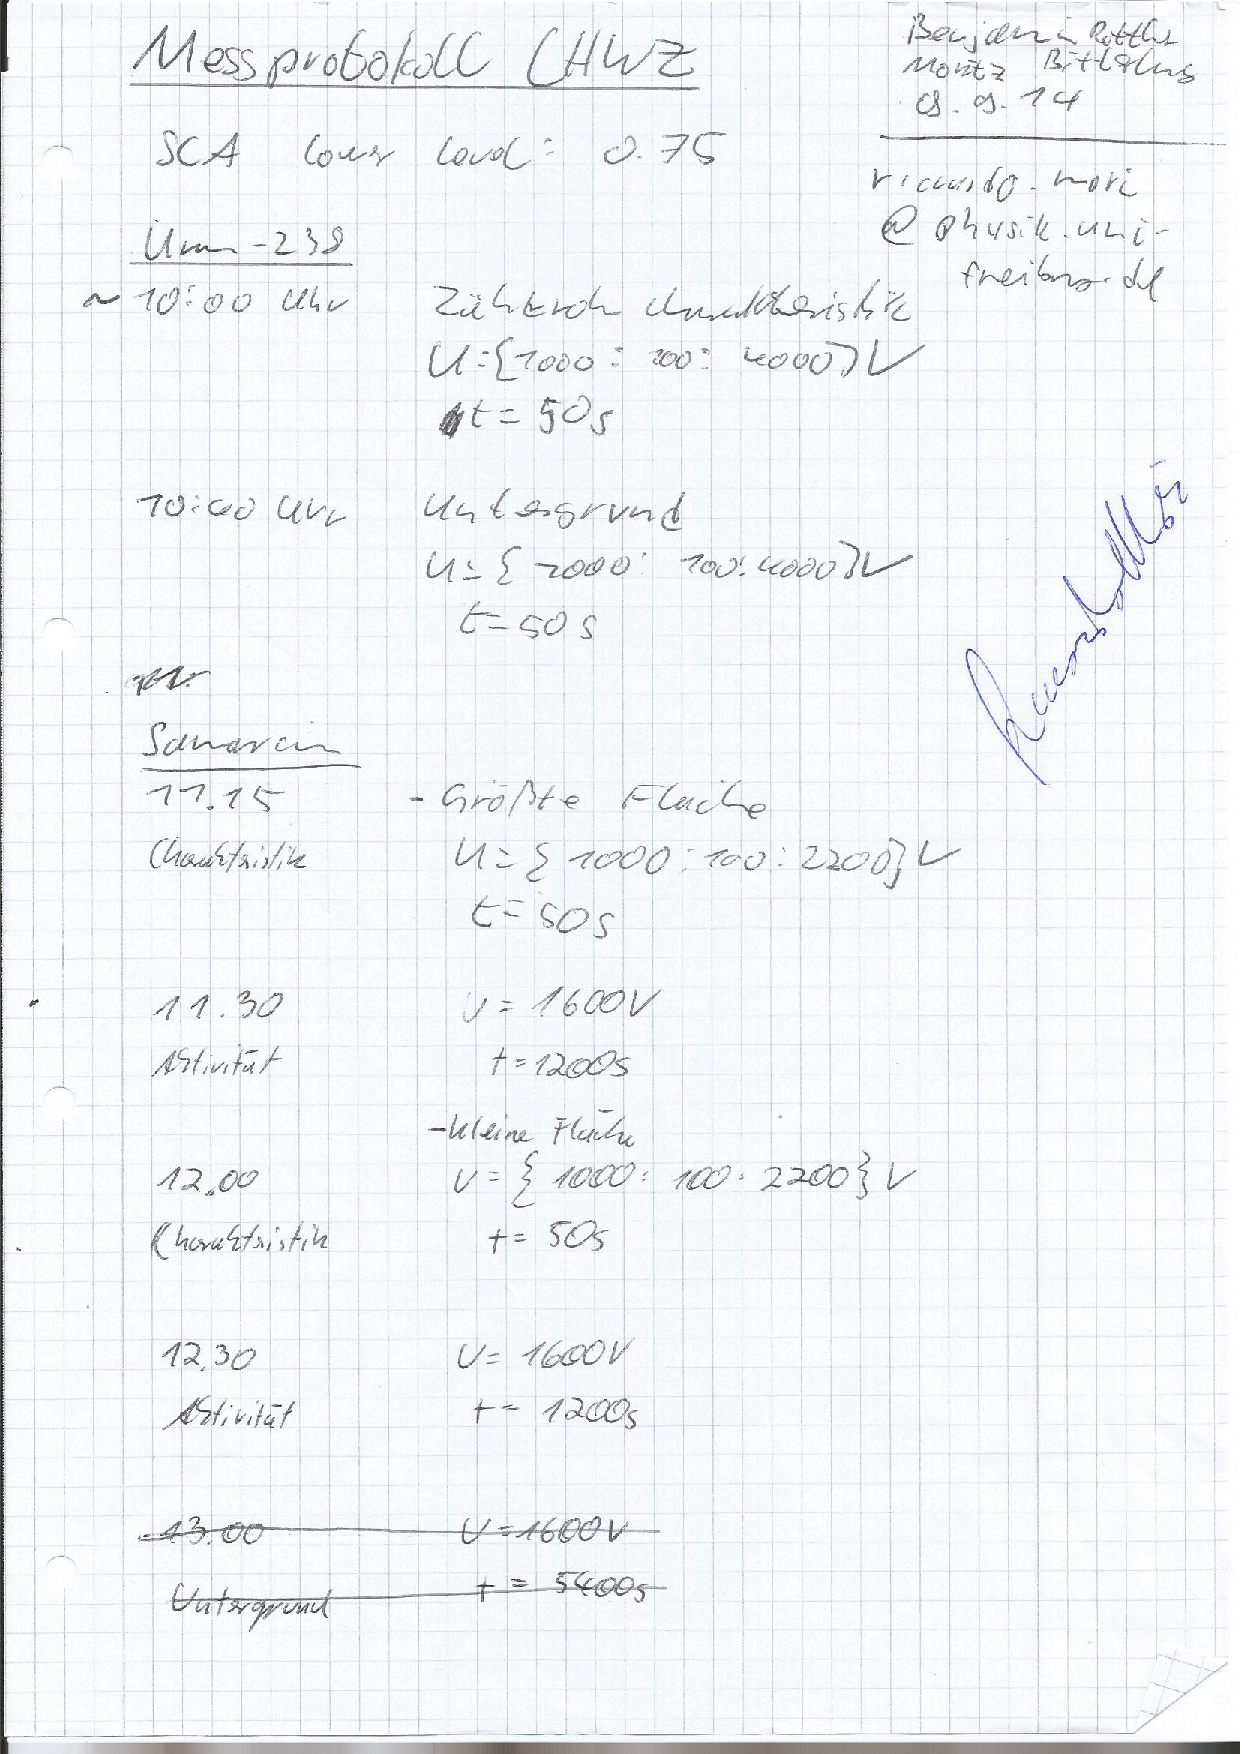
\includepdf[pages={-}]{../data/protokoll.pdf}


\end{document}